\documentclass[11pt]{article}
\usepackage[letterpaper,margin=0.7in]{geometry}
\usepackage[T1]{fontenc}
\usepackage{lmodern}
\usepackage{microtype}
\usepackage{amsmath}
\usepackage{graphicx}
\usepackage{subcaption}
\usepackage{float}
\usepackage{booktabs}
\usepackage{listings}
\usepackage[section]{placeins}
\usepackage{xcolor}
\usepackage{hyperref}
\hypersetup{pdftitle={Computational Photography HW3},pdfauthor={Chung-Ting Tsai},colorlinks=true,linkcolor=blue!45!black,urlcolor=blue!45!black}
\graphicspath{{figures/}}
\captionsetup{font=small,labelfont=bf,skip=6pt}
\setlength{\parindent}{0pt}
\setlength{\parskip}{6pt}
\setlength{\textfloatsep}{12pt plus 2pt minus 2pt}
\setlength{\intextsep}{10pt plus 2pt minus 2pt}
\lstset{basicstyle=\ttfamily\small,breaklines=true,frame=single,rulecolor=\color{black!20},backgroundcolor=\color{black!3},aboveskip=6pt,belowskip=6pt}
% Placeholder for text to write. Search for \todo before submitting.
\newcommand{\todo}[1]{{\color{red!70!black}\textbf{[TODO:} \textit{#1}\textbf{]}}}
\begin{document}
\begin{center}
{\Large\bfseries 15-663 Computational Photography}\\[4pt]
{\large Homework 3: Flash/No-Flash Photography}\\[4pt]
Chung-Ting Tsai
\end{center}

%======================================================================
\section{Bilateral filtering}
%======================================================================
\subsection*{Implementation}
All images are normalized to $[0,1]$ and each color channel is filtered separately. I implemented two bilateral filters that take a source image and a guide image, so the same function performs basic filtering (\texttt{src = guide}) and joint filtering (\texttt{src} $=A$, \texttt{guide} $=F$):
\begin{itemize}\setlength{\itemsep}{0pt}
\item \texttt{bilateral\_filtering}: the PiecewiseBilateral algorithm of Durand and Dorsey, with linear interpolation between intensity segments using \texttt{scipy.interpolate.interpn}. Following the hint, I extend the intensity range by a margin of $\lambda=0.001$ on each side.
\item \texttt{brute\_force\_bilateral}: a direct evaluation over a circular window of radius $3\sigma_s$. Its cost grows with $\sigma_s$ but not with $1/\sigma_r$, which makes it practical for the very small $\sigma_r$ used for joint filtering. On test crops it agrees with the piecewise filter to a mean absolute difference below $10^{-3}$.
\end{itemize}

\subsection*{Discussion}
\begin{itemize}\setlength{\itemsep}{2pt}
\item \textbf{Basic bilateral filtering.} Increasing either $\sigma_s$ or $\sigma_r$ gives a blurrier result (Figure~\ref{fig:p1sweepbase}). At large $\sigma_r$, the difference images contain strand structure in addition to grain, which means scene detail is removed along with the noise (Figure~\ref{fig:p1sweepbaseres}). I chose $\sigma_s=16$ and $\sigma_r=0.05$, which removes most of the noise while keeping the image sharp.

\item \textbf{Joint bilateral filtering.} I first used $\sigma_s=4$ and $\sigma_r=0.05$, but the lamp strands became very blurry, much more than in $A^{Base}$ (Figures~\ref{fig:p1sweepnr} and~\ref{fig:p1sweepnrres}). As Figure~\ref{fig:p1jbfdiag} shows, this is likely because the edges in the ambient and flash images differ: the strands are lit from behind by the lamp in the ambient image and from the front in the flash image, and the joint filter only preserves the edges of the flash image. Following Petschnigg et al., who set $\sigma_r$ to $0.1\%$ of the intensity range, I reduced $\sigma_r$ to $0.001$. The strands become noticeably sharper, but more noise remains (Figure~\ref{fig:p1brute}). The piecewise implementation is impractical at this $\sigma_r$: it would need about 1000 segments, and storing all of them exceeds the available memory, so I used the brute-force implementation instead.

\item \textbf{Advantage of joint bilateral filtering.} Compared with basic bilateral filtering, which uses only the ambient image, the final result preserves the texture of the wall and the grooves of the pan much better (Figure~\ref{fig:p1stages}).

\item \textbf{Detail transfer.} I used $\epsilon=0.02$, the value used in the paper. Because the detail layer is the ratio between the flash image and its smoothed version, it adds the fine detail of the flash image back to $A^{NR}$ (Figure~\ref{fig:p1detail}). $F^{Base}$ must be smoothed with a moderate $\sigma_r$; with $\sigma_r=0.001$ on these 8-bit images, $F^{Base}$ equals $F$ and the detail layer is 1 everywhere.

\item \textbf{Masking.} Some regions that do not look like flash shadows are still detected, because their flash intensity is lower than the ISO-normalized ambient intensity (Figure~\ref{fig:p1masks}), for example parts of the dark pans and the gaps between the strands. Petschnigg et al.\ list four causes of such false detections: surfaces with near-zero albedo, distant surfaces the flash does not reach, noise, and inter-reflection. The black pans fit the first case, and the gaps between the strands are lit mainly by the lamp itself rather than the flash. The rendered 8-bit images are also only approximately linear after inverse sRGB gamma, which affects the comparison.

\item \textbf{Preferred result.} Personally, I prefer the basic bilateral result, even though it blurs the wall. The full pipeline recovers more of the wall texture (Figures~\ref{fig:p1stages} and~\ref{fig:p1diffs}), but I find the result less aesthetically pleasing.
\end{itemize}

\begin{table}[!htbp]
\centering
\small
\begin{tabular}{lll}
\toprule
Method & Implementation & Selected parameters \\
\midrule
Basic bilateral ($A^{Base}$) & piecewise & $\sigma_s=16$, $\sigma_r=0.05$ \\
Joint bilateral ($A^{NR}$) & brute force & $\sigma_s=4$, $\sigma_r=0.001$ \\
Detail transfer ($A^{Detail}$) & piecewise ($F^{Base}$) & $F^{Base}$: $\sigma_s=16$, $\sigma_r=0.05$; $\epsilon=0.02$ \\
Mask-based merging ($A^{Final}$) & --- & $\tau_{shad}=0$; $Y_F>0.95$; open $3$, close $5$, dilate $3$; feather $\sigma=2$ \\
\bottomrule
\end{tabular}
\caption{Selected parameters. The feathered mask exceeds 0.5 on 3.9\% of the pixels.}
\label{tab:p1params}
\end{table}

\clearpage
\subsection*{Input pair}
\begin{figure}[H]
\centering
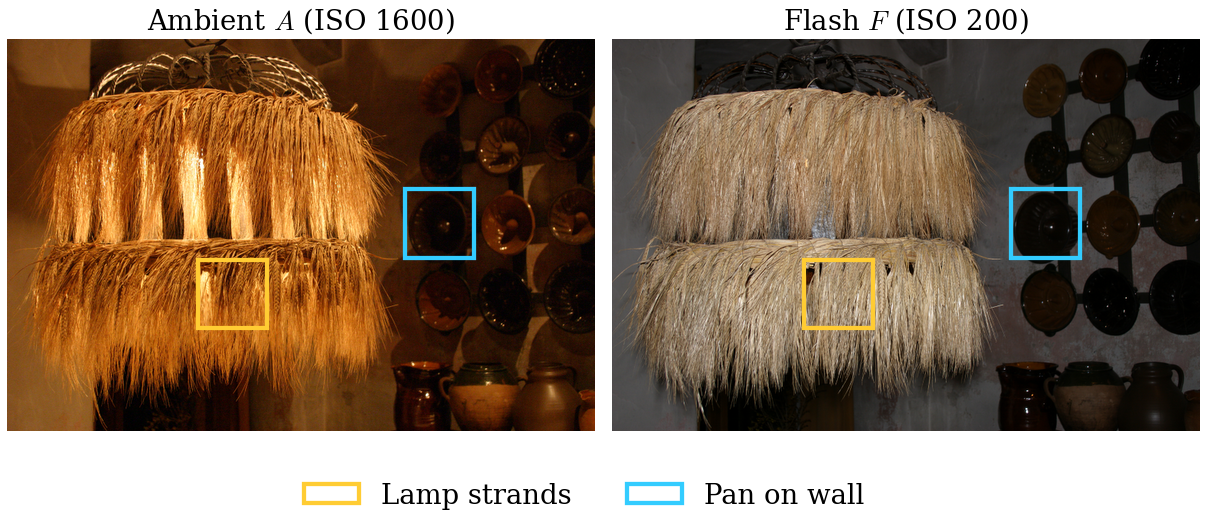
\includegraphics[width=\linewidth]{p1_inputs.png}
\caption{Input pair. The boxes mark the zoom regions used in the later figures: the lamp strands (fine texture) and a pan on the wall (a dark, noisy region with flash shadows and specular highlights).}
\label{fig:p1inputs}
\end{figure}

\subsection*{Basic bilateral filtering ($A^{Base}$)}
\begin{figure}[H]
\centering
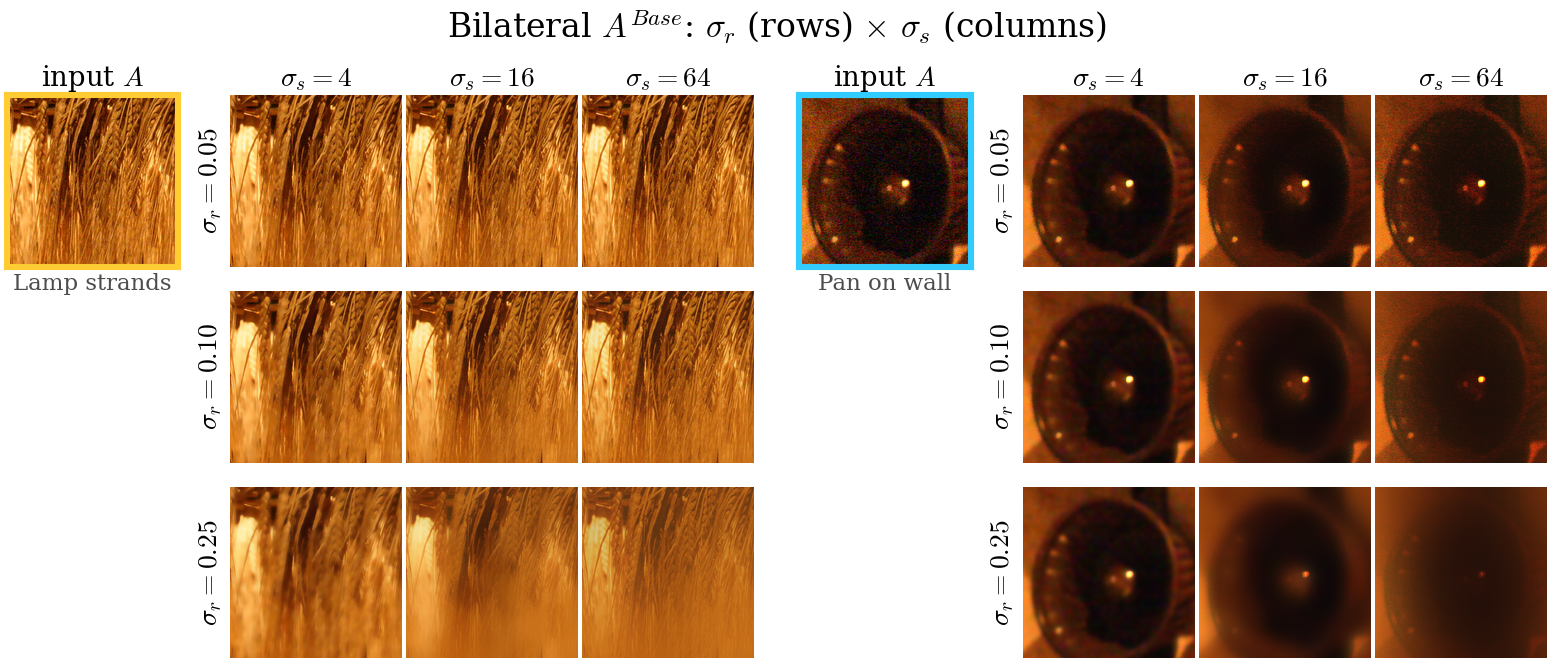
\includegraphics[width=\linewidth]{p1_sweep_base.png}
\caption{Basic bilateral filtering of the ambient image for $\sigma_s\in\{4,16,64\}$ and $\sigma_r\in\{0.05,0.10,0.25\}$ (selected: $\sigma_s=16$, $\sigma_r=0.05$). The pan crop is displayed with a $2.5\times$ brightness gain.}
\label{fig:p1sweepbase}
\end{figure}
\begin{figure}[H]
\centering
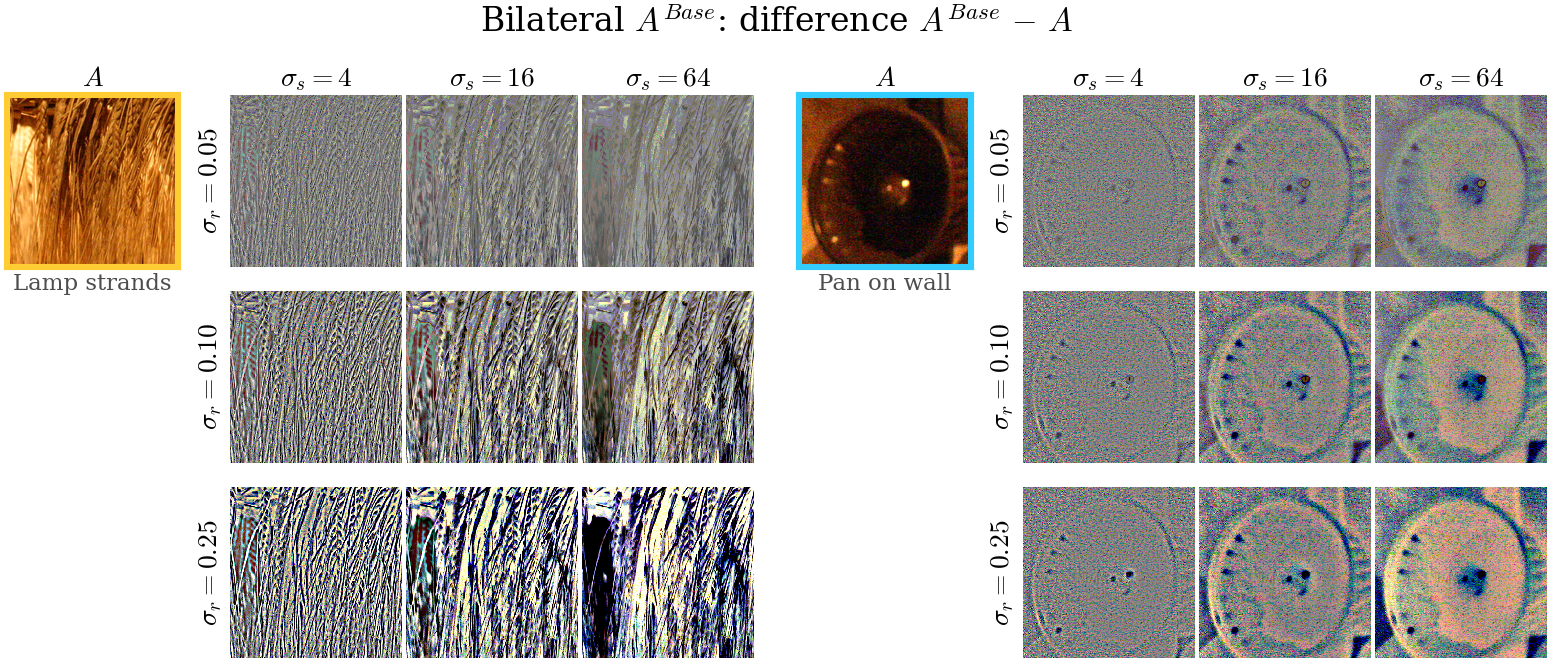
\includegraphics[width=\linewidth]{p1_sweep_base_residual.png}
\caption{Difference images $A^{Base}-A$ for the grid of Figure~\ref{fig:p1sweepbase}, shown per RGB channel as $0.5+(A^{Base}-A)/0.16$ (mid-gray: no change). Grain-like differences are removed noise; structure that follows strands or edges is removed scene detail.}
\label{fig:p1sweepbaseres}
\end{figure}

\subsection*{Joint bilateral filtering ($A^{NR}$)}
\begin{figure}[H]
\centering
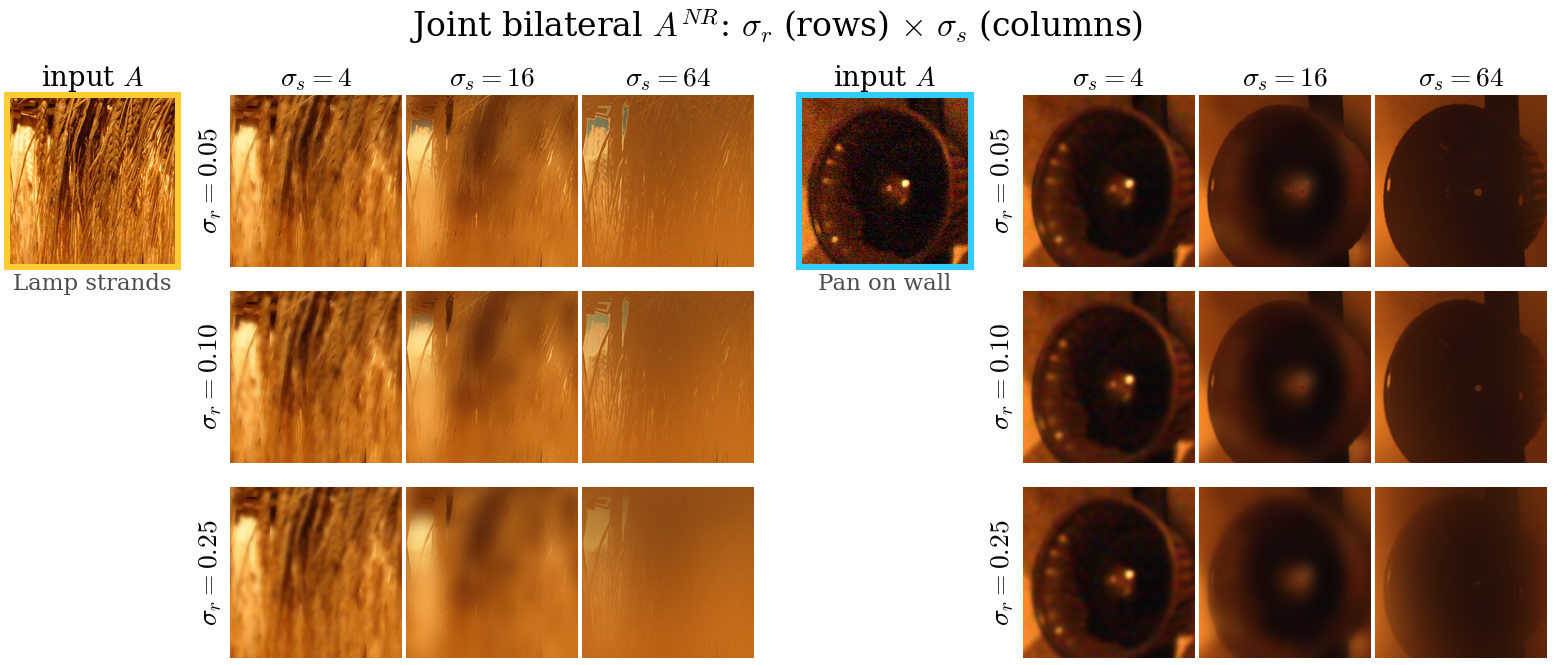
\includegraphics[width=\linewidth]{p1_sweep_nr.png}
\caption{Joint bilateral filtering of the ambient image with the flash image as the guide (piecewise implementation, suggested range $\sigma_r\in[0.05,0.25]$). The pan crop is displayed with a $2.5\times$ brightness gain.}
\label{fig:p1sweepnr}
\end{figure}
\begin{figure}[H]
\centering
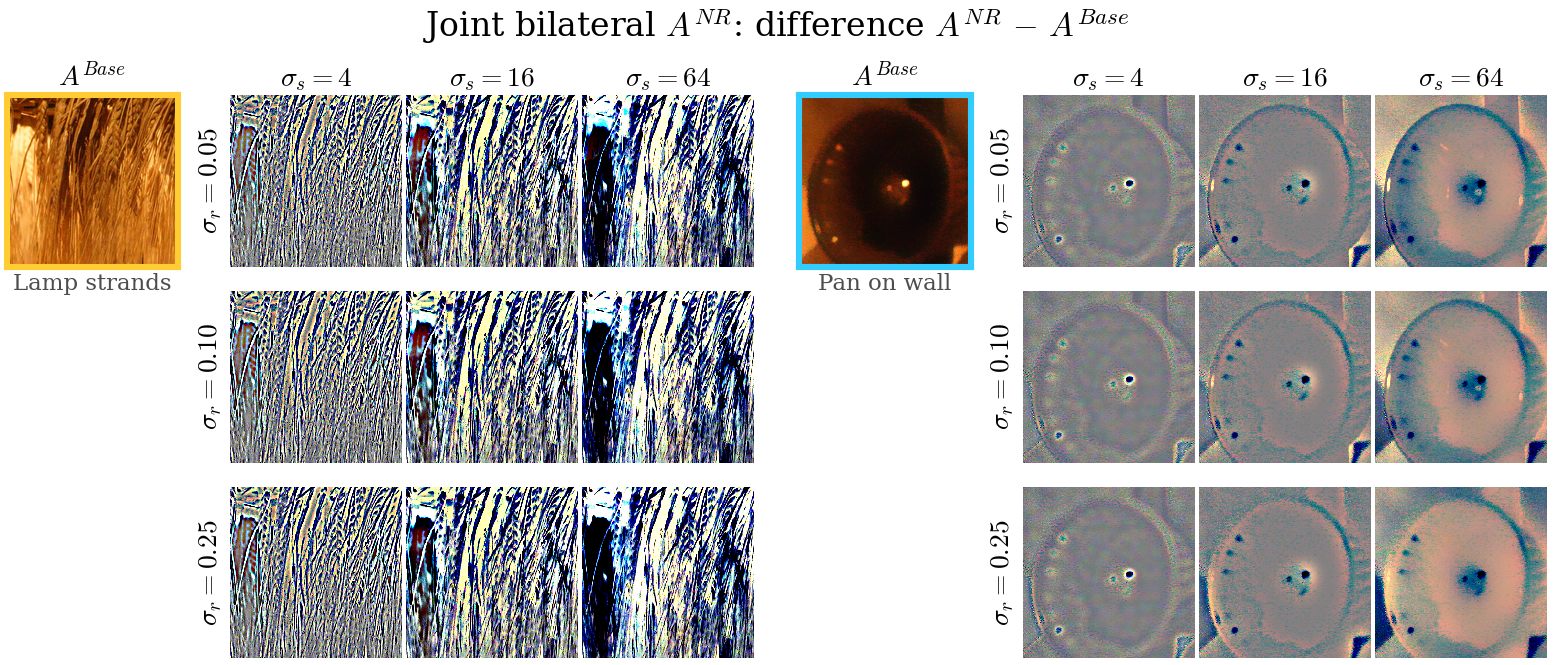
\includegraphics[width=\linewidth]{p1_sweep_nr_residual.png}
\caption{Difference images $A^{NR}-A^{Base}$ for the grid of Figure~\ref{fig:p1sweepnr}, with $A^{Base}$ fixed at the selected setting ($\sigma_s=16$, $\sigma_r=0.05$; left column). Shown per RGB channel (mid-gray: no change). Strong structure in the strands means $A^{NR}$ smooths much more than $A^{Base}$.}
\label{fig:p1sweepnrres}
\end{figure}
\begin{figure}[H]
\centering
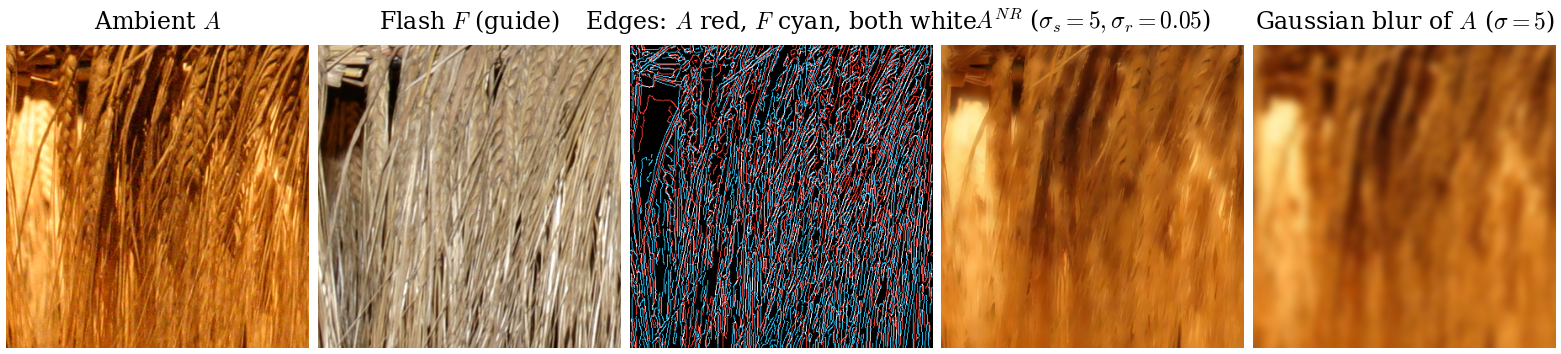
\includegraphics[width=\linewidth]{p1_jbf_diagnosis.png}
\caption{Why the strands blur. Ambient and flash images, their Canny edges (ambient red, flash cyan, shared white), $A^{NR}$ ($\sigma_s=5$, $\sigma_r=0.05$), and a Gaussian blur of $A$ ($\sigma=5$). The strands are back-lit in $A$ and front-lit in $F$: about 31\% of the ambient edges have no flash edge within one pixel, so the joint filter averages across them and $A^{NR}$ is close to the Gaussian blur. Shifting $F$ by its best offset (2\,px) reduced the mean difference between $A^{NR}$ and $A$ by only 8\%, so misalignment is a minor factor.}
\label{fig:p1jbfdiag}
\end{figure}
\begin{figure}[H]
\centering
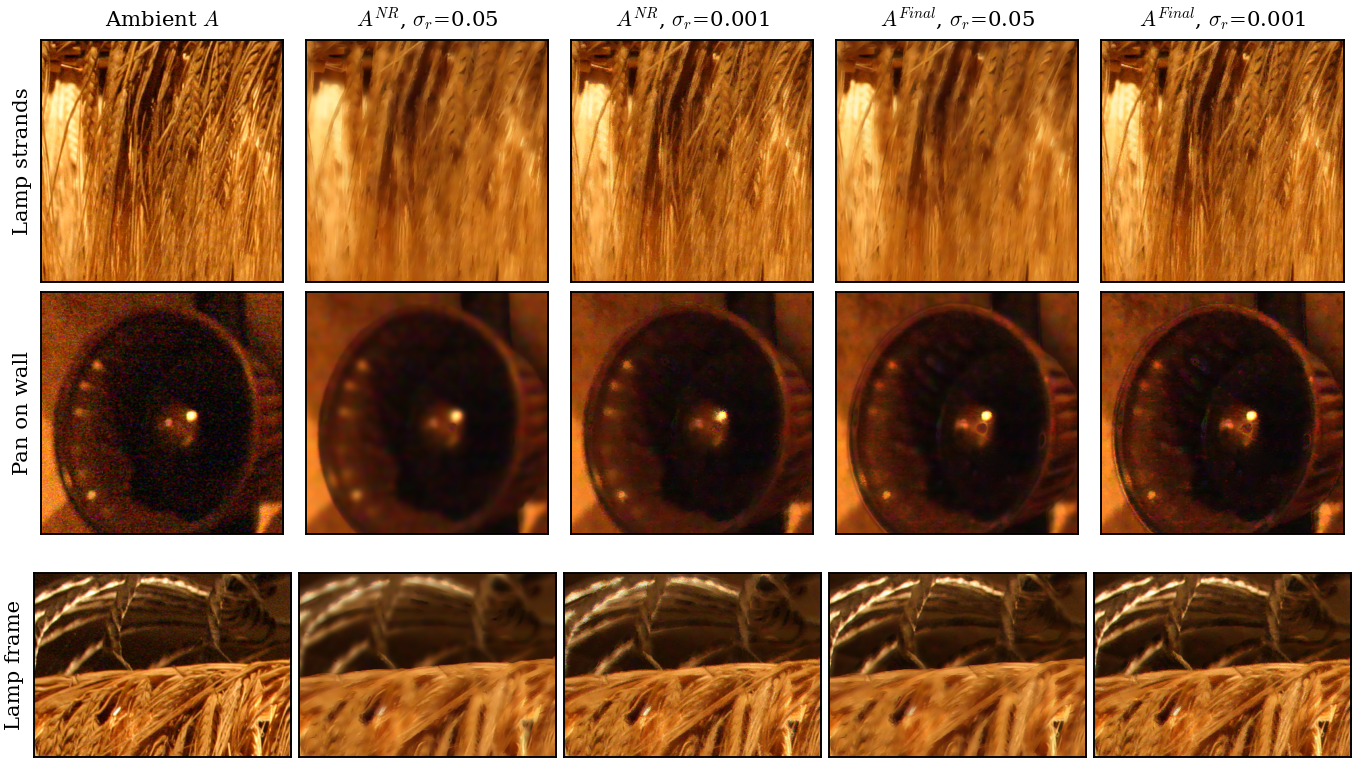
\includegraphics[width=\linewidth]{p1_jbf_brute_sigma_r.png}
\caption{Small $\sigma_r$. $A^{NR}$ and $A^{Final}$ with $\sigma_s=4$ and $\sigma_r=0.05$ (piecewise) or $\sigma_r=0.001$ (brute force; Petschnigg et al.\ use $0.1\%$ of the range, which would need about 1000 piecewise segments). The pan crop is displayed with a $2.5\times$ brightness gain.}
\label{fig:p1brute}
\end{figure}

\subsection*{Detail transfer ($A^{Detail}$)}
\begin{figure}[H]
\centering
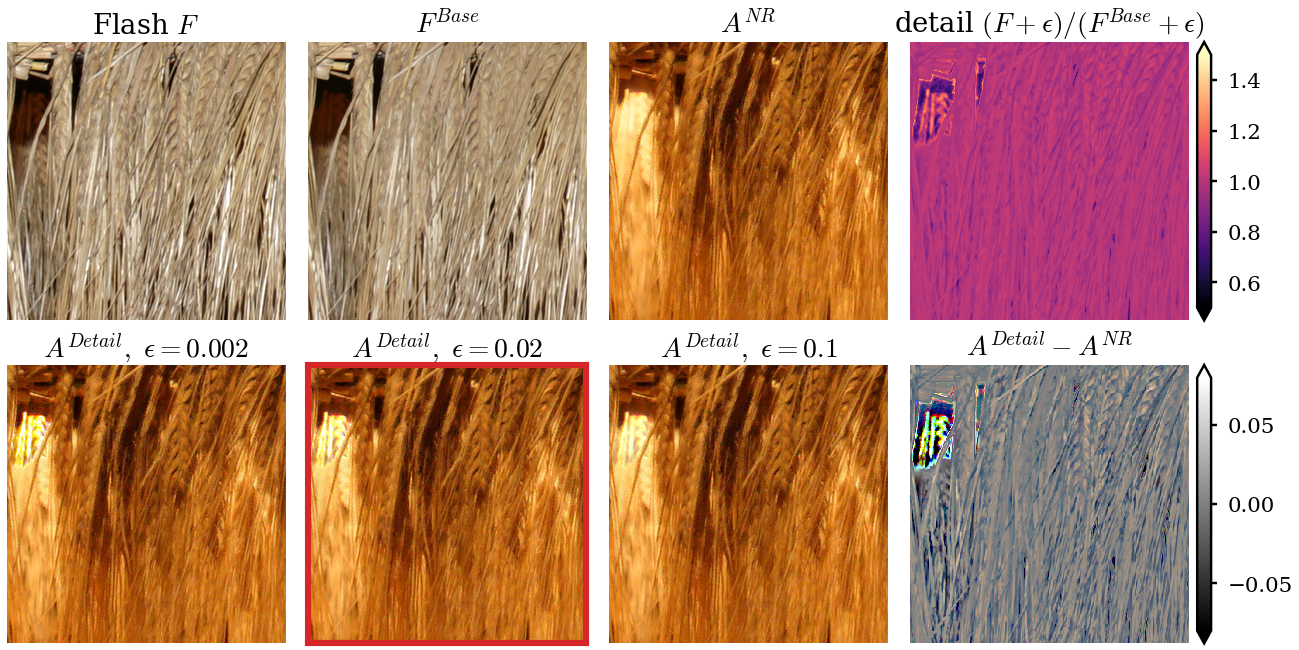
\includegraphics[width=\linewidth]{p1_detail_transfer.png}
\caption{Detail transfer $A^{Detail}=A^{NR}(F+\epsilon)/(F^{Base}+\epsilon)$ on the strand crop, with $F^{Base}$ from basic bilateral filtering of the flash image ($\sigma_s=16$, $\sigma_r=0.05$). Top: flash image, $F^{Base}$, $A^{NR}$, and the luma of the detail layer. Bottom: $A^{Detail}$ for three values of $\epsilon$ (selected value outlined in red) and the difference $A^{Detail}-A^{NR}$ per RGB channel (mid-gray: no change).}
\label{fig:p1detail}
\end{figure}

\subsection*{Shadow and specularity masking ($A^{Final}$)}
\begin{figure}[H]
\centering
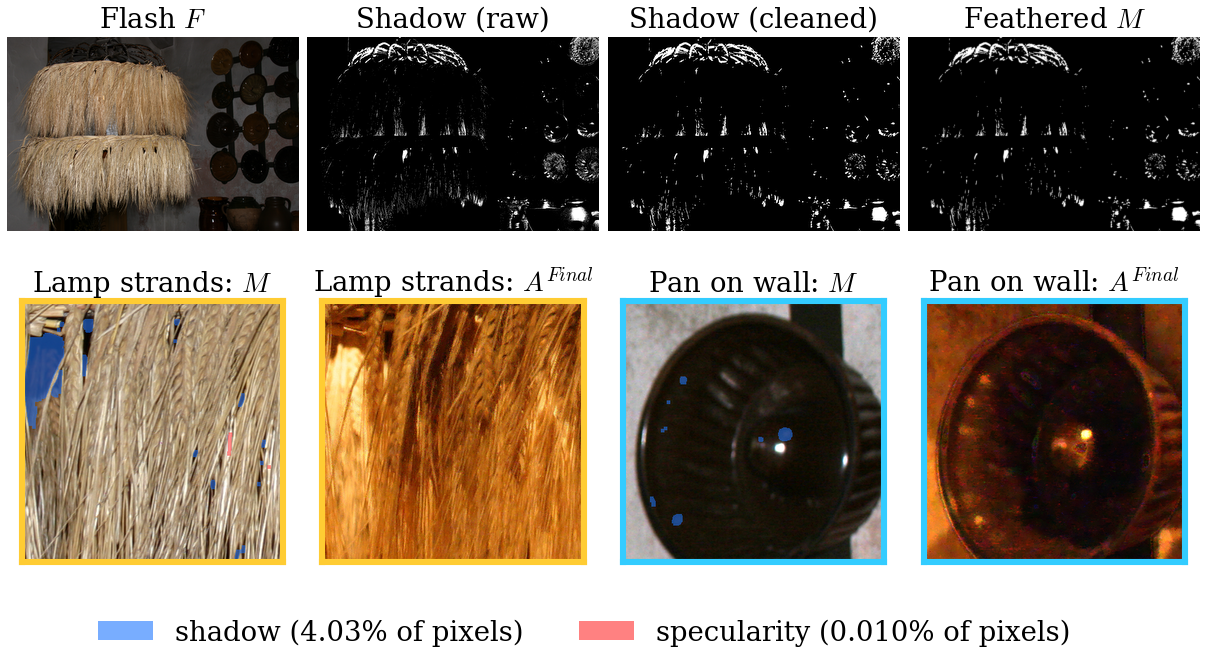
\includegraphics[width=\linewidth]{p1_masks.png}
\caption{Mask computed on linear luminance with the ambient image ISO-normalized to the flash image (ISO 1600 vs.\ 200): shadow where $Y_F-\tfrac{200}{1600}Y_A\le0$, specularity where $Y_F>0.95$. Each mask is cleaned with a $3\times3$ opening, a $5\times5$ closing and a $3\times3$ dilation; the union is feathered with a Gaussian ($\sigma=2$). Top: flash image, raw and cleaned shadow masks, and the feathered mask $M$. Bottom: shadow (blue) and specularity (red) masks and $A^{Final}$ in the two zoom regions (pan crop shown with a $2.5\times$ gain).}
\label{fig:p1masks}
\end{figure}

\subsection*{Comparison of the four methods}
\begin{figure}[H]
\centering
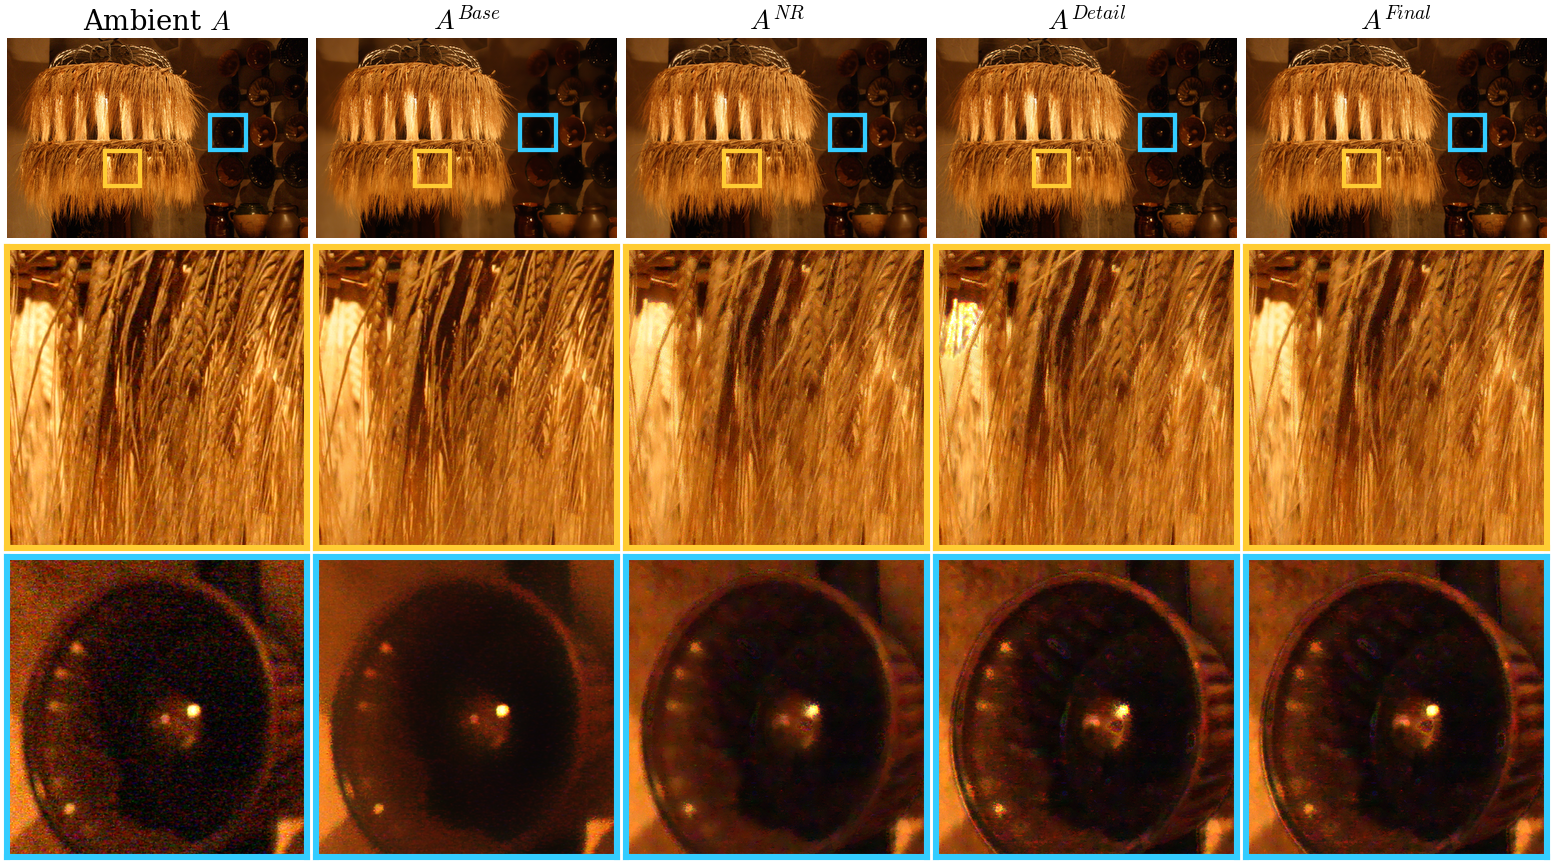
\includegraphics[width=\linewidth]{p1_stages.png}
\caption{Ambient input and the four results with the selected parameters (Table~\ref{tab:p1params}). The pan crop is displayed with a $2.5\times$ brightness gain.}
\label{fig:p1stages}
\end{figure}
\begin{figure}[H]
\centering
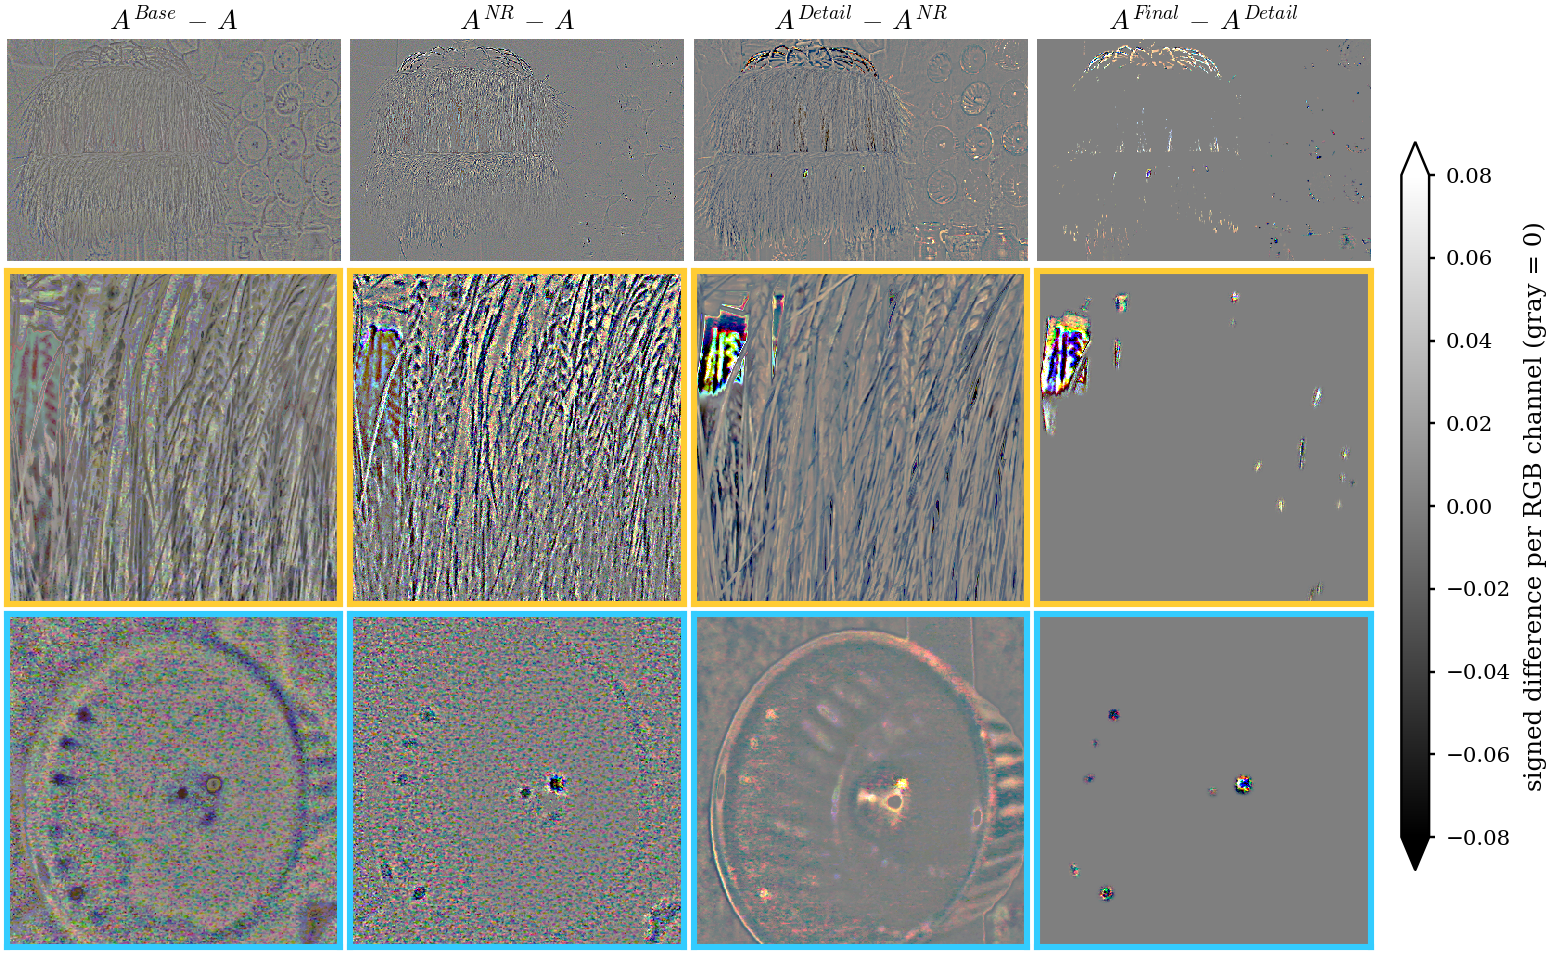
\includegraphics[width=\linewidth]{p1_stage_differences.png}
\caption{Signed difference images between methods, shown per RGB channel as $0.5+d/0.16$ (mid-gray: no change; values beyond $\pm0.08$ are clipped).}
\label{fig:p1diffs}
\end{figure}

%======================================================================
\clearpage
\section{Gradient-domain processing}
%======================================================================
\subsection*{Implementation}
Images are normalized to $[0,1]$ and each RGB channel is processed separately. I implemented three operators that are reused throughout:
\begin{itemize}\setlength{\itemsep}{0pt}
\item \texttt{grad}: backward differences (\texttt{np.diff} with zero prepended), returning the $y$ and $x$ derivatives.
\item \texttt{divergence}: forward differences (\texttt{np.diff} with zero appended), so that $\mathrm{div}(\nabla I)$ equals the Laplacian at every interior pixel.
\item \texttt{laplacian}: convolution with the kernel of Equation~(9) using \texttt{scipy.signal.convolve2d} (\texttt{mode='same'}, zero fill).
\end{itemize}
\texttt{gradient\_cgd} implements Algorithm~1 with Dirichlet boundary conditions: the mask $B$ is 0 on the outermost pixels and 1 elsewhere, and the iteration stops when $\sqrt{\langle r,r\rangle}<\epsilon$ or after $N$ iterations. \texttt{fused\_gradient} computes the coherency map $M$ (Equation~(4)), the saturation weight $w_s$ (Equation~(5), normalized to $[0,1]$) and the fused field $\nabla\Phi^*$ (Equation~(6)), which is then integrated by passing its divergence to the solver.

\subsection*{Discussion}
\begin{itemize}\setlength{\itemsep}{2pt}
\item \textbf{Re-integration.} The solver recovers the original image from its Laplacian: with $\epsilon=10^{-3}$ the maximum error is 0.0019 after about 1280 iterations, and with $\epsilon=10^{-6}$ it drops to $1.7\times10^{-6}$ after about 2200 iterations (Figure~\ref{fig:p2reint}).

\item \textbf{Saturation weight.} In $w_s=\tanh\big(\sigma(\Phi'-\tau_s)\big)$, $\tau_s$ sets the intensity above which the flash image is treated as saturated, and $\sigma$ sets how sharply the weight switches around this threshold. A smaller $\sigma$ gives a softer transition, so after normalization $w_s$ is larger over a wider range of intensities; more ambient gradients are then used and the result becomes darker. A smaller $\tau_s$ marks more of the bright flash region as saturated. In the highlight region, however, the differences between the settings are small to the eye (Figure~\ref{fig:p2sweep}); the most visible one is a faint gray haze for $\sigma=10$, $\tau_s=0.7$. I therefore kept the values of Agrawal et al., $\sigma=40$ and $\tau_s=0.9$.

\item \textbf{Boundary conditions and initialization.} The boundary values change the result smoothly across the whole image (Figure~\ref{fig:p2bc}). For example, the bottom boundary of the flash image is brighter, so with flash boundary values the neck and shoulders become brighter, and the left side gets a cyan tint. The initialization does not change the result (the four initializations agree to within 0.004 for a fixed boundary), only the convergence speed (Figure~\ref{fig:p2conv}): with ambient boundary values, the average of the two images converges fastest (about 900 iterations), the ambient or flash image is slightly faster than the zero image (about 1170--1200 vs.\ 1250 iterations).

\item \textbf{Final result.} The fused image (Figure~\ref{fig:p2final}) removes the flash highlight on the painting, where $w_s$ selects the ambient gradients (Figure~\ref{fig:p2weights}), while the face keeps the detail of the flash image. A few dark spots remain where the highlight was.
\end{itemize}

\begin{table}[!htbp]
\centering
\small
\begin{tabular}{ll}
\toprule
Step & Selected parameters \\
\midrule
Re-integration test & $\epsilon=10^{-3}$, $N=3000$; zero initialization; boundary from $I$ \\
Saturation weight & $\sigma=40$, $\tau_s=0.9$ (values of Agrawal et al.) \\
Fusion & $\epsilon=10^{-3}$, $N=3000$; initialization: average of $a$ and $\Phi'$; boundary: ambient \\
\bottomrule
\end{tabular}
\caption{Selected parameters for gradient-domain fusion.}
\label{tab:p2params}
\end{table}

\clearpage
\subsection*{Differentiate and re-integrate an image}
\begin{figure}[H]
\centering
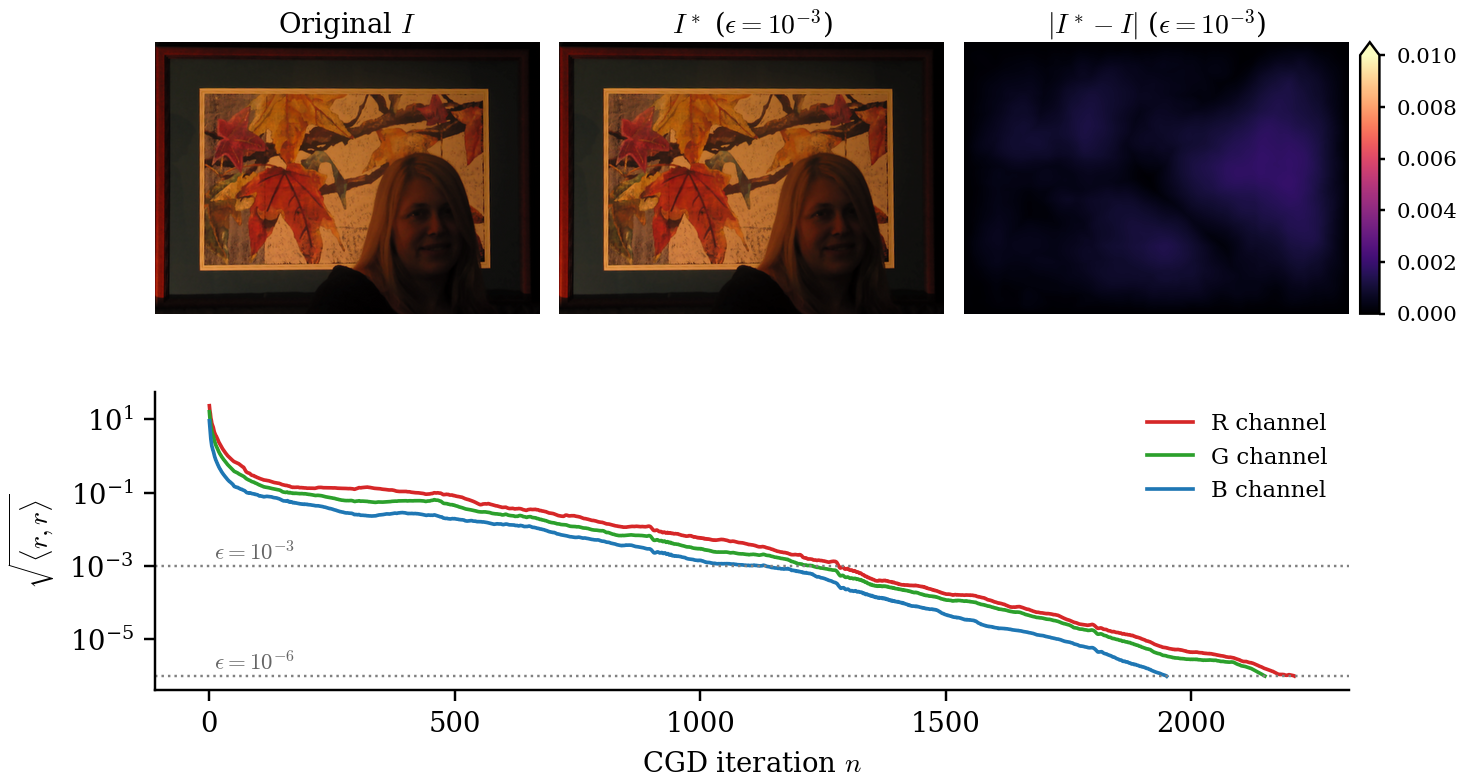
\includegraphics[width=\linewidth]{p2_reintegration.png}
\caption{Re-integration of the ambient image from its Laplacian, with zero initialization and Dirichlet boundary values from $I$. Top: original $I$, the result $I^*$ with $\epsilon=10^{-3}$ (about 1280 iterations), and the absolute error (maximum over channels; maximum error 0.0019). Bottom: residual norm per iteration for each channel; with $\epsilon=10^{-6}$ (about 2200 iterations) the maximum error is $1.7\times10^{-6}$.}
\label{fig:p2reint}
\end{figure}

\subsection*{Create the fused gradient field}
\begin{figure}[H]
\centering
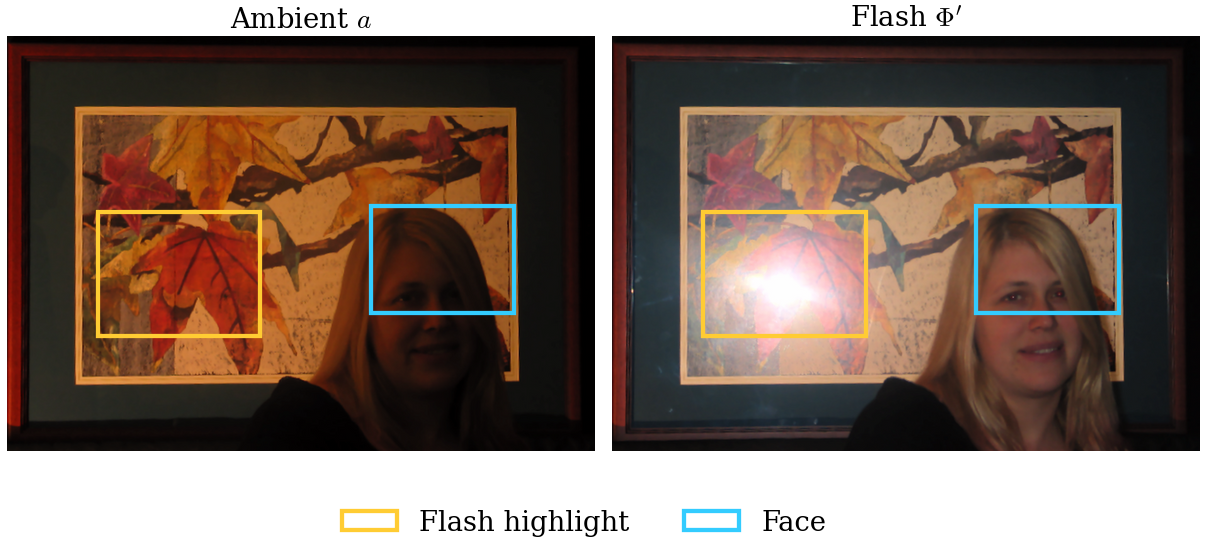
\includegraphics[width=\linewidth]{p2_inputs.png}
\caption{Input pair: ambient image $a$ and flash image $\Phi'$. The boxes mark the zoom regions used later: the flash highlight on the painting and the face.}
\label{fig:p2inputs}
\end{figure}
\begin{figure}[H]
\centering
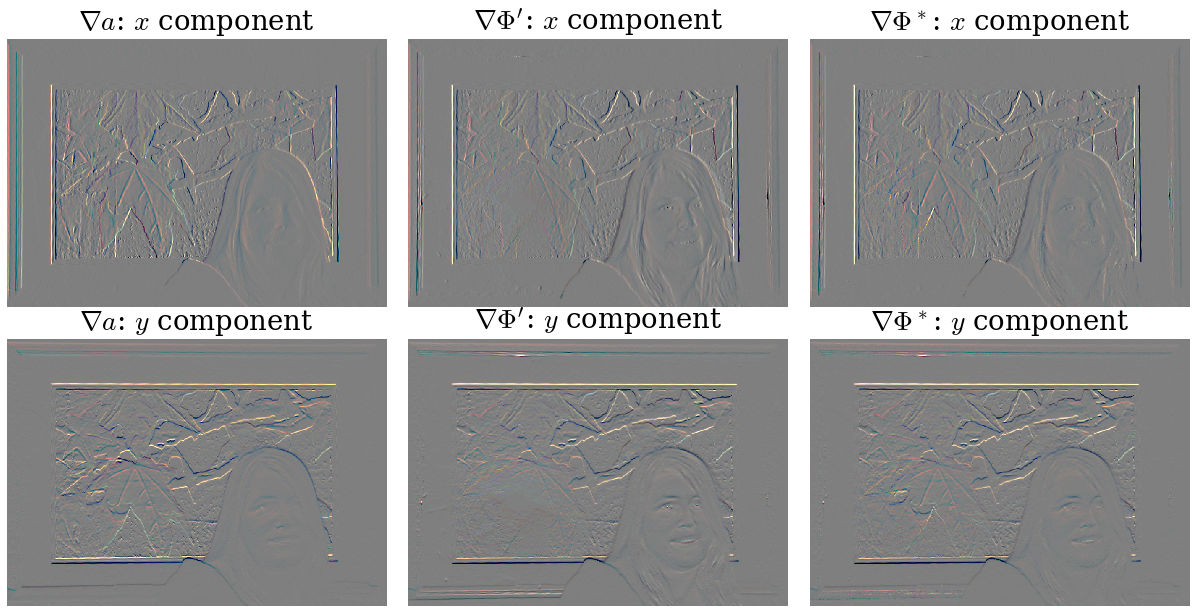
\includegraphics[width=\linewidth]{p2_gradients.png}
\caption{Gradient fields of the ambient image, the flash image and the fused field ($\sigma=40$, $\tau_s=0.9$), shown per RGB channel as $0.5+g/0.3$ (mid-gray: zero gradient).}
\label{fig:p2grad}
\end{figure}
\begin{figure}[H]
\centering
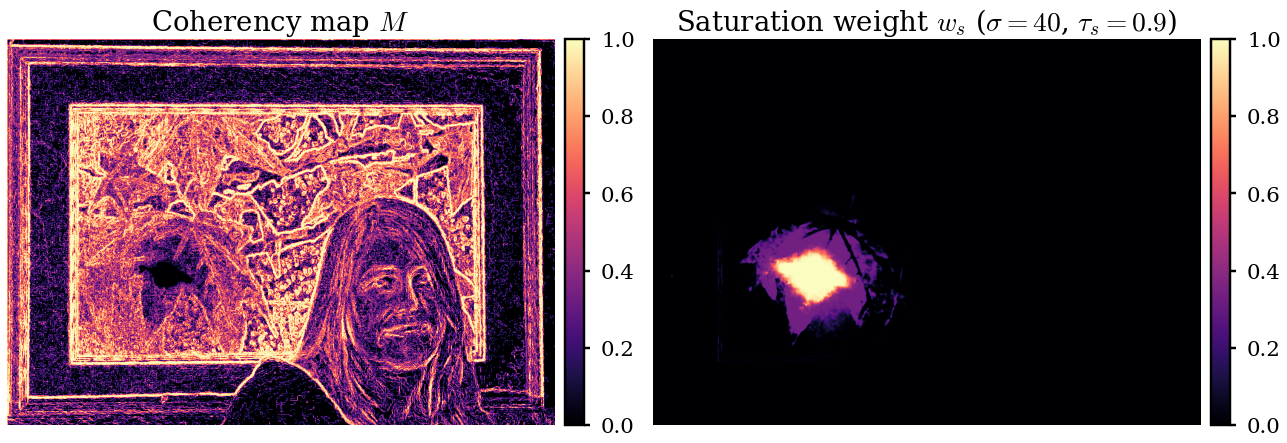
\includegraphics[width=\linewidth]{p2_weights.png}
\caption{Coherency map $M$ and normalized saturation weight $w_s$ (both averaged over the RGB channels). $M$ is close to 1 where the ambient and flash gradients are parallel; $w_s$ is close to 1 in the saturated flash highlight, where the ambient gradients are used.}
\label{fig:p2weights}
\end{figure}
\begin{figure}[H]
\centering
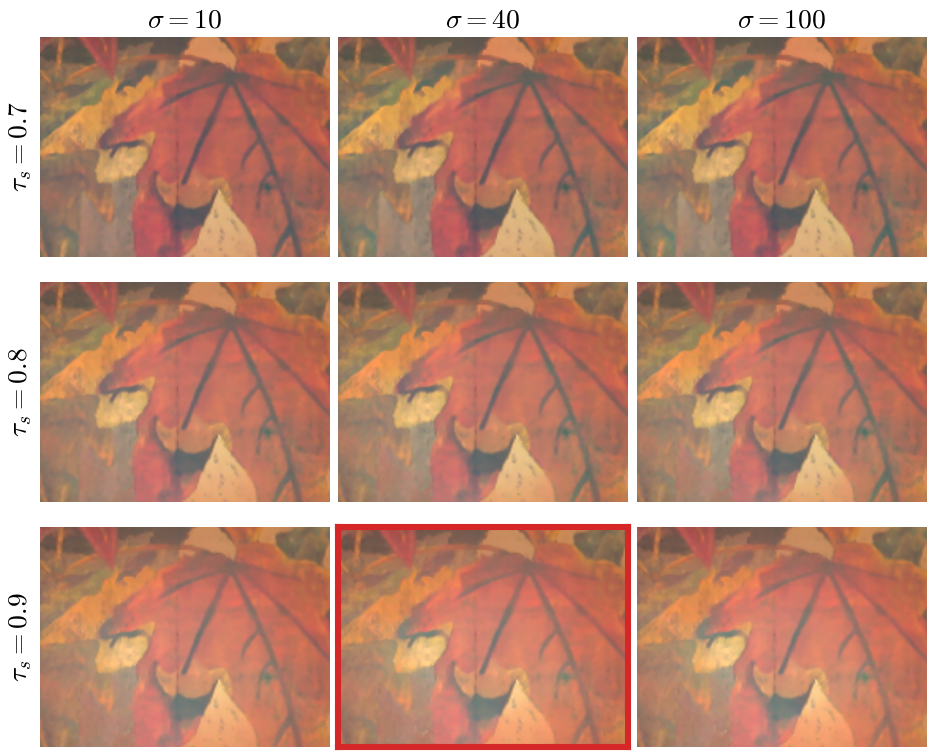
\includegraphics[width=0.75\linewidth]{p2_sweep.png}
\caption{Fused result in the highlight region for $\sigma\in\{10,40,100\}$ and $\tau_s\in\{0.7,0.8,0.9\}$ (average initialization, ambient boundary). The values of Agrawal et al.\ are outlined in red.}
\label{fig:p2sweep}
\end{figure}

\subsection*{Boundary conditions and initialization}
\begin{figure}[H]
\centering
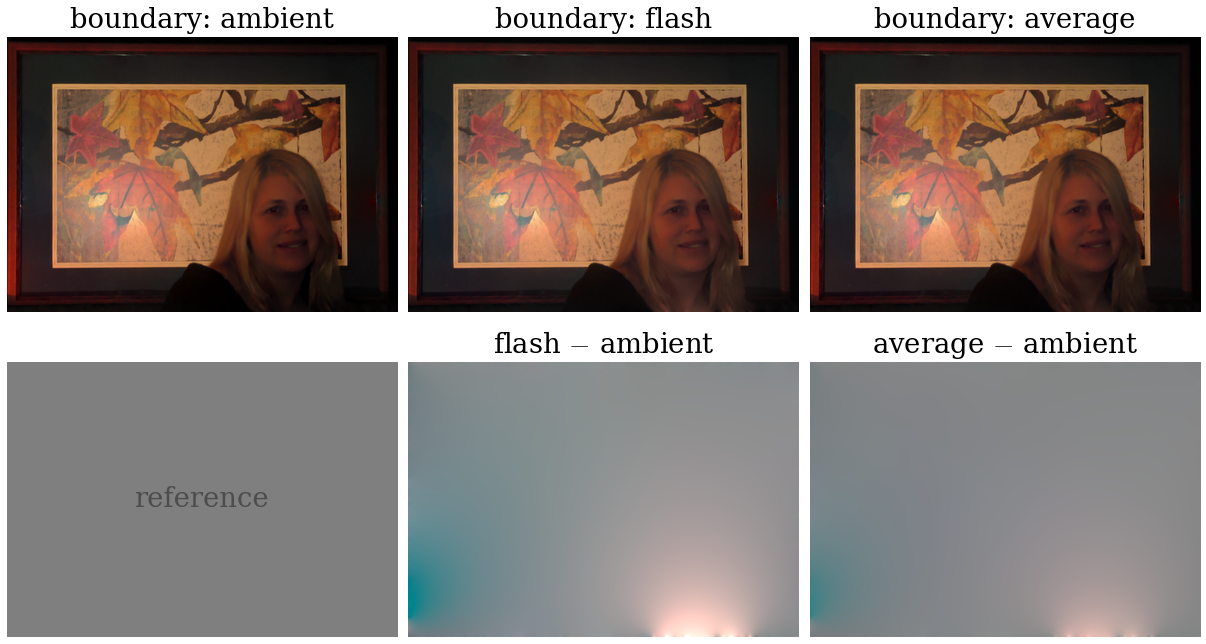
\includegraphics[width=\linewidth]{p2_bc_init.png}
\caption{Fused results for ambient, flash and average boundary values (average initialization). Bottom: differences from the ambient-boundary result, per RGB channel as $0.5+d/0.3$ (mid-gray: no change). The boundary values change the result smoothly across the image, by up to 0.3 near the edges. For a fixed boundary, the four initializations give the same result to within 0.004.}
\label{fig:p2bc}
\end{figure}
\begin{figure}[H]
\centering
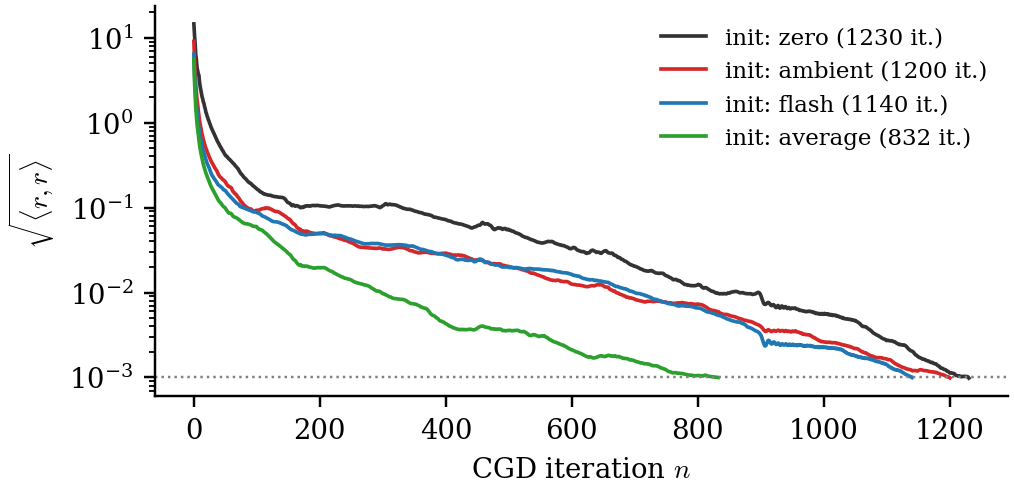
\includegraphics[width=0.72\linewidth]{p2_convergence.png}
\caption{Residual norm per iteration for the four initializations (ambient boundary, green channel), with the number of iterations needed to reach $\epsilon=10^{-3}$.}
\label{fig:p2conv}
\end{figure}

\subsection*{Final result}
\begin{figure}[H]
\centering
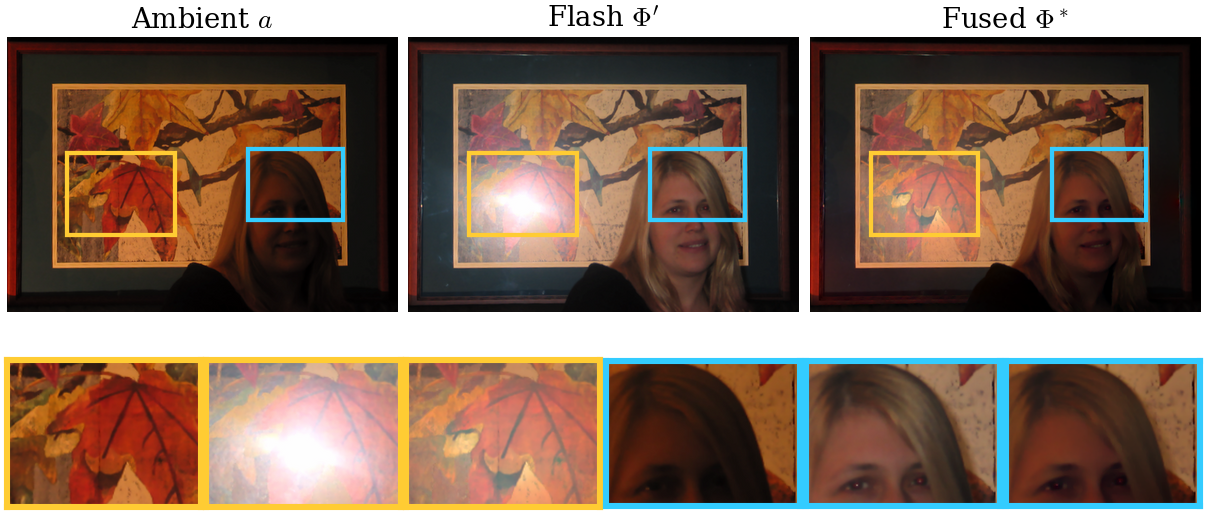
\includegraphics[width=\linewidth]{p2_final.png}
\caption{Ambient image, flash image and fused result $\Phi^*$ with the selected parameters (Table~\ref{tab:p2params}), with zoomed views of the flash highlight (yellow) and the face (blue).}
\label{fig:p2final}
\end{figure}

%======================================================================
\clearpage
\section{Capture your own flash/no-flash pairs}
%======================================================================
\subsection*{Pair 1: bilateral-filtering denoising}

\subsubsection*{Capture}
Both photographs were taken with a Nikon D3500 on a tripod at $6000\times4000$ pixels, with the same shutter speed (1/4\,s) and aperture ($f/4$). The ambient image was taken at ISO 1600 under a single desk lamp, and the flash image at ISO 200 with the built-in flash. The scene contains fine, low-contrast textures in dark regions (a knit scarf and a knit beanie), where the noise of the ambient image is strongest.

\subsubsection*{Implementation}
I used the same pipeline and parameters as for the lamp pair (Table~\ref{tab:p3params}). The camera stayed on a tripod between the two exposures, so the images are used as captured, without alignment.

\subsubsection*{Discussion}
\begin{itemize}\setlength{\itemsep}{0pt}
\item \textbf{Scene design.} To build a scene where joint bilateral filtering is clearly better than basic bilateral filtering, I placed a knit scarf and a knit beanie in front of the camera. Both are dark and have fine, low-contrast textures, so in the high-ISO ambient image these regions are noisy and their texture is comparable in contrast to the noise.

\item \textbf{Basic vs.\ joint bilateral filtering.} As shown in Figure~\ref{fig:p3stages}, applying the basic bilateral filter to the ambient image removes the noise but also blurs the knit texture and the logo on the scarf. With the flash image as the guide, joint bilateral filtering keeps these fine textures while removing the noise. The difference images confirm this (Figure~\ref{fig:p3diffs}): $A^{Base}-A$ contains the logo and the folds of the beanie, i.e.\ removed scene detail, while $A^{NR}-A$ is mostly grain, i.e.\ removed noise.

\item \textbf{Detail transfer and masking.} Detail transfer adds a little more of the knit texture from the flash image (Figure~\ref{fig:p3detail}). The scene has almost no flash shadows or specularities, so the mask covers only 0.02\% of the pixels and $A^{Final}$ is nearly identical to $A^{Detail}$.
\end{itemize}

\begin{table}[!htbp]
\centering
\small
\begin{tabular}{lll}
\toprule
Method & Implementation & Selected parameters \\
\midrule
Basic bilateral ($A^{Base}$) & piecewise & $\sigma_s=16$, $\sigma_r=0.05$ \\
Joint bilateral ($A^{NR}$) & brute force & $\sigma_s=4$, $\sigma_r=0.001$ \\
Detail transfer ($A^{Detail}$) & piecewise ($F^{Base}$) & $F^{Base}$: $\sigma_s=16$, $\sigma_r=0.05$; $\epsilon=0.02$ \\
Mask-based merging ($A^{Final}$) & --- & ISO 1600 vs.\ 200; $\tau_{shad}=0$; $Y_F>0.95$; open 3, close 5, dilate 3; feather $\sigma=2$ \\
\bottomrule
\end{tabular}
\caption{Parameters for my first pair (same as for the lamp pair). The mask covers only 0.02\% of the pixels, so $A^{Final}$ is nearly identical to $A^{Detail}$.}
\label{tab:p3params}
\end{table}

\clearpage
\subsubsection*{Results}
\begin{figure}[H]
\centering
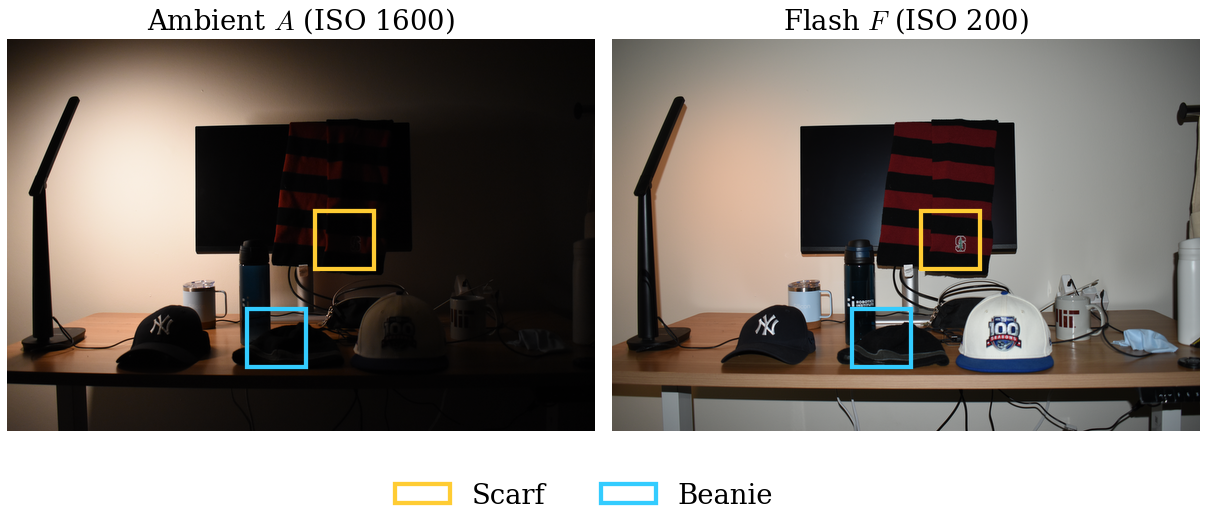
\includegraphics[width=\linewidth]{p3_desk_inputs.png}
\caption{My first pair: ambient image (ISO 1600, lit by a desk lamp) and flash image (ISO 200), both 1/4\,s at $f/4$. The boxes mark the zoom regions: the knit scarf with its logo and the knit beanie.}
\label{fig:p3inputs}
\end{figure}
\begin{figure}[H]
\centering
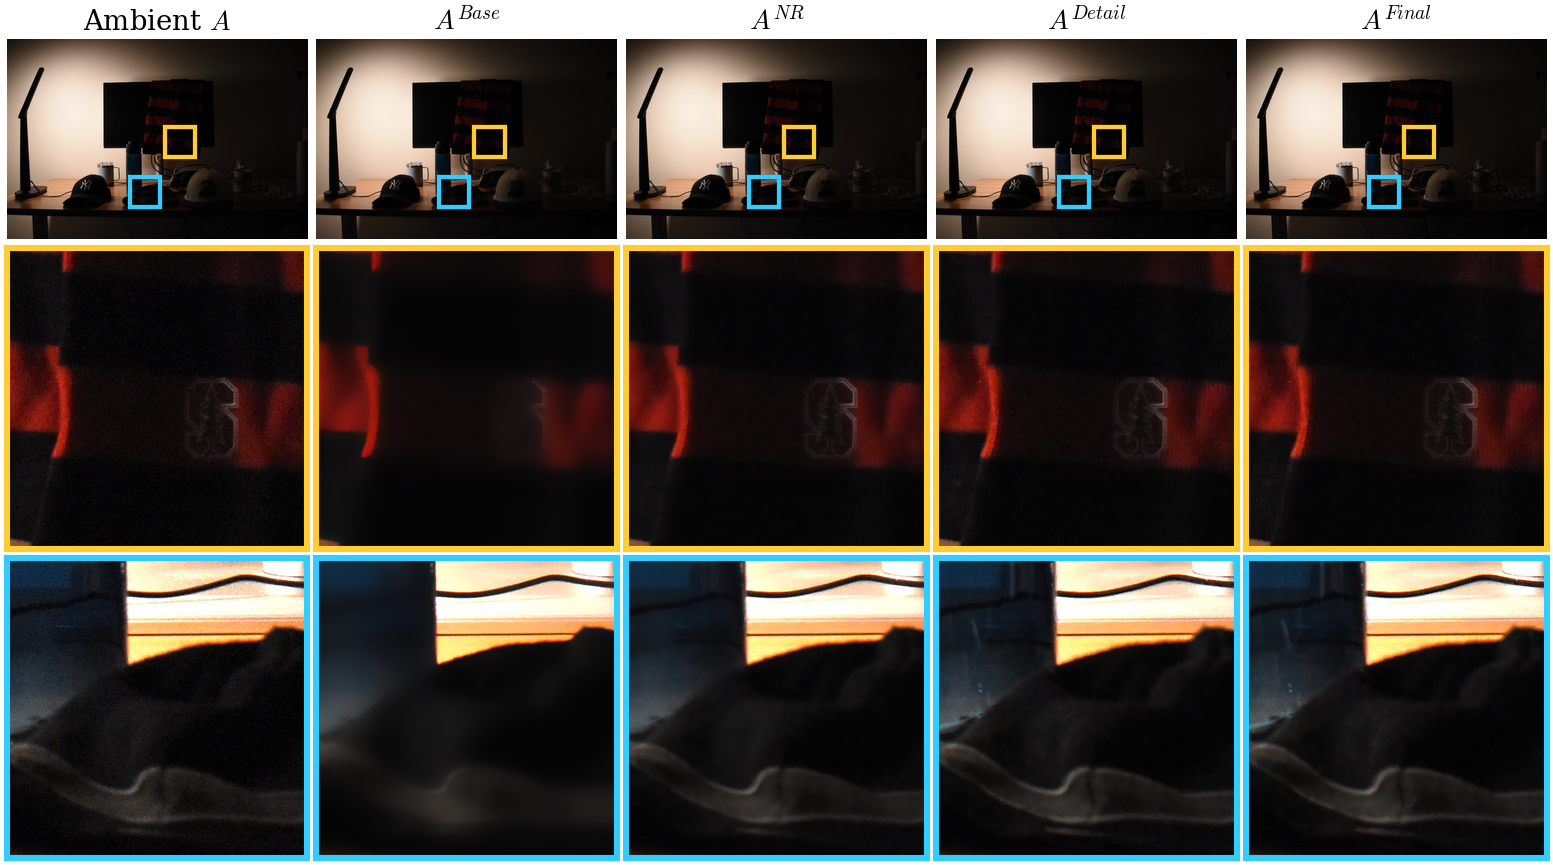
\includegraphics[width=\linewidth]{p3_desk_stages.png}
\caption{Ambient input and the four results. Both crops are displayed with a $3\times$ brightness gain. $A^{Base}$ blurs the knit texture and the logo; $A^{NR}$ and $A^{Detail}$ keep them while removing the noise.}
\label{fig:p3stages}
\end{figure}
\begin{figure}[H]
\centering
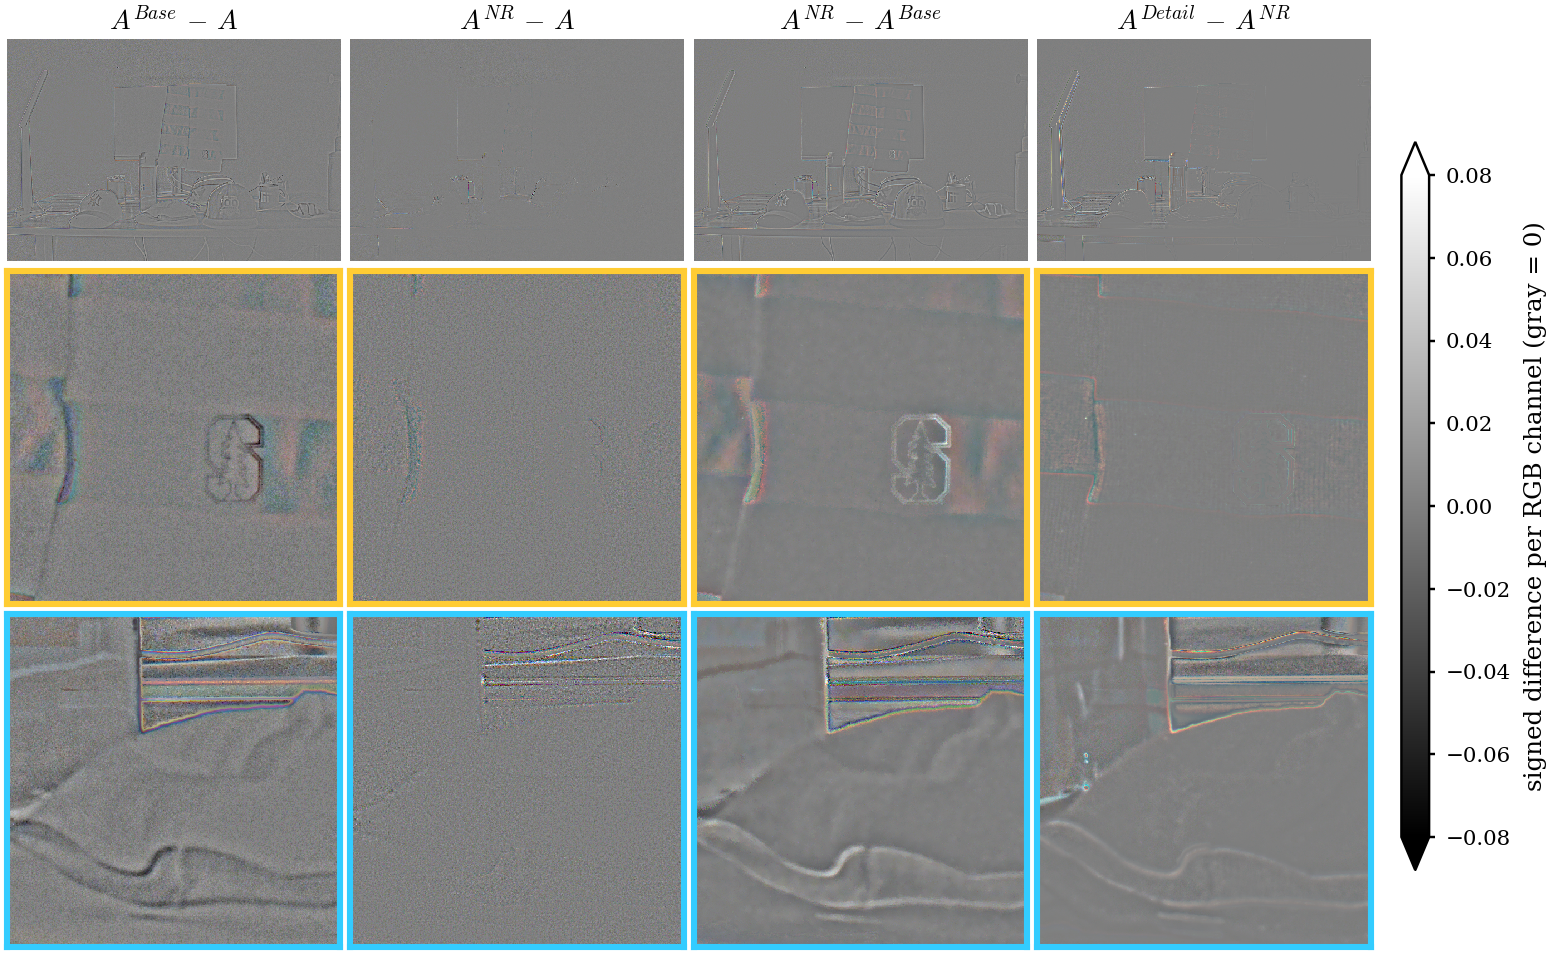
\includegraphics[width=\linewidth]{p3_desk_stage_differences.png}
\caption{Signed difference images, shown per RGB channel as $0.5+d/0.16$ (mid-gray: no change). $A^{Base}-A$ contains the logo and the folds of the beanie (removed scene detail), while $A^{NR}-A$ is mostly grain (removed noise). $A^{NR}-A^{Base}$ shows the detail that joint filtering keeps.}
\label{fig:p3diffs}
\end{figure}
\begin{figure}[H]
\centering
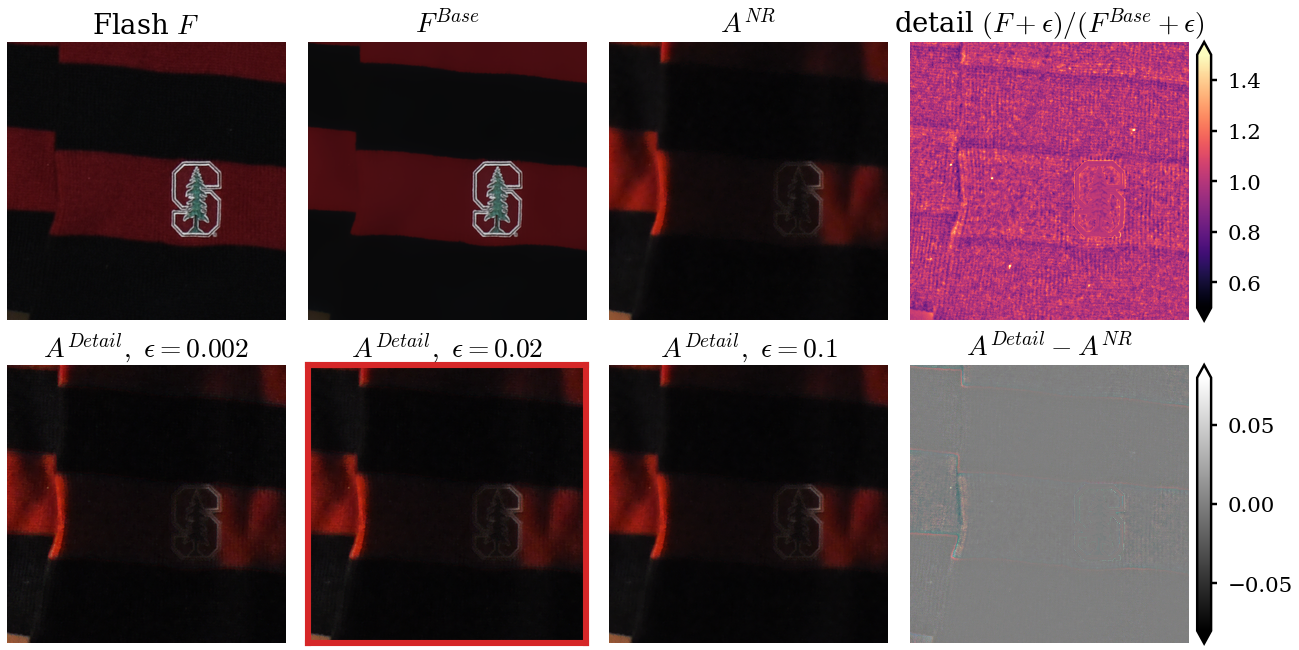
\includegraphics[width=\linewidth]{p3_desk_detail_transfer.png}
\caption{Detail transfer on the scarf crop: flash image, $F^{Base}$, $A^{NR}$ and the luma of the detail layer (top); $A^{Detail}$ for three values of $\epsilon$ (selected value outlined in red) and the difference $A^{Detail}-A^{NR}$ (bottom). Ambient-based panels are displayed with a $3\times$ brightness gain.}
\label{fig:p3detail}
\end{figure}

\clearpage
\subsection*{Pair 2: gradient-domain fusion}

\subsubsection*{Capture}
Both photographs were taken with the Nikon D3500 on a tripod at ISO 200 and $f/4$. The ambient image was exposed for 4\,s with the desk lamp aimed at an acrylic card stand, so the cards are well lit while the mug and the bottle in front stay dark. The flash image was exposed for 1/4\,s with the built-in flash, which lights the mug and the bottle but creates a saturated glare on the acrylic and a specular streak on the glossy mug.

\subsubsection*{Implementation}
I used the gradient-domain fusion of Part~2 (Table~\ref{tab:p3p2params}). To keep the CGD solve fast, both images are downsampled to $1500\times1000$ pixels. As for Pair~1, the camera stayed on a tripod, so the images are used without alignment.

\subsubsection*{Discussion}

\begin{itemize}\setlength{\itemsep}{0pt}
\item \textbf{Scene design.} To demonstrate gradient-domain fusion, I designed the lighting so that each image fails in a different region (Figure~\ref{fig:p3p2inputs}). The desk lamp lights the cards behind the acrylic, so they are well exposed in the ambient image, while the mug and the bottle in front stay dark. The flash lights the mug and the bottle, but creates a glare on the acrylic and a streak on the glossy mug.

\item \textbf{Choice of $\tau_s$.} With the parameters of Agrawal et al.\ ($\sigma=40$, $\tau_s=0.9$), the glare on the acrylic is not fully removed: only its saturated core is covered by $w_s$, and a pale blob remains from the unsaturated halo around it. Lowering $\tau_s$ to 0.7 extends $w_s$ over the halo, which removes most of the glare (Figure~\ref{fig:p3p2tau}). The fused result keeps the lamp-lit cards from the ambient image and the mug and the bottle from the flash image (Figure~\ref{fig:p3p2final}).

\item \textbf{Limitations.} The streak on the mug remains, because the mug is black in the ambient image, so there are no ambient gradients to replace it with. In addition, with $\tau_s=0.7$ the saturation weight also covers the bright front of the table (Figure~\ref{fig:p3p2weights}); there, the dark and noisy ambient gradients are used, which produces a color tint.
\end{itemize}

\begin{table}[!htbp]
\centering
\small
\begin{tabular}{ll}
\toprule
Step & Selected parameters \\
\midrule
Preprocessing & downsample to $1500\times1000$; no alignment (tripod) \\
Saturation weight & $\sigma=40$, $\tau_s=0.7$ \\
Fusion & $\epsilon=10^{-3}$, $N=5000$; initialization: average of $a$ and $\Phi'$; boundary: ambient \\
\bottomrule
\end{tabular}
\caption{Parameters for my second pair.}
\label{tab:p3p2params}
\end{table}

\clearpage
\subsubsection*{Results}
\begin{figure}[H]
\centering
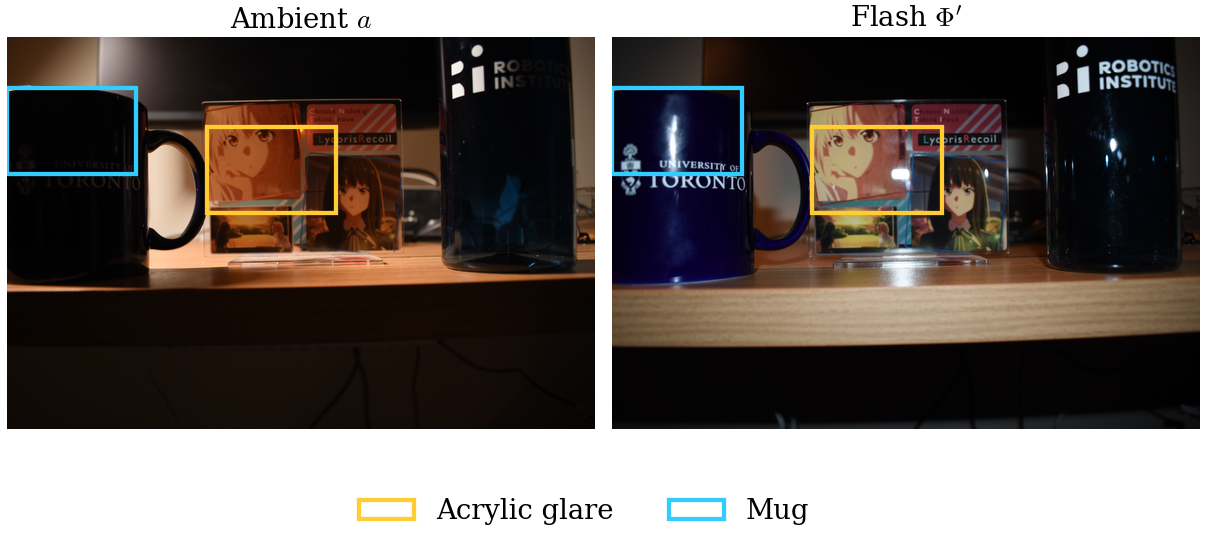
\includegraphics[width=\linewidth]{p3_glare_inputs.png}
\caption{My second pair: ambient image (ISO 200, 4\,s, lit by a desk lamp aimed at the cards) and flash image (ISO 200, 1/4\,s), both at $f/4$. The boxes mark the zoom regions: the flash glare on the acrylic and the specular streak on the mug.}
\label{fig:p3p2inputs}
\end{figure}
\begin{figure}[H]
\centering
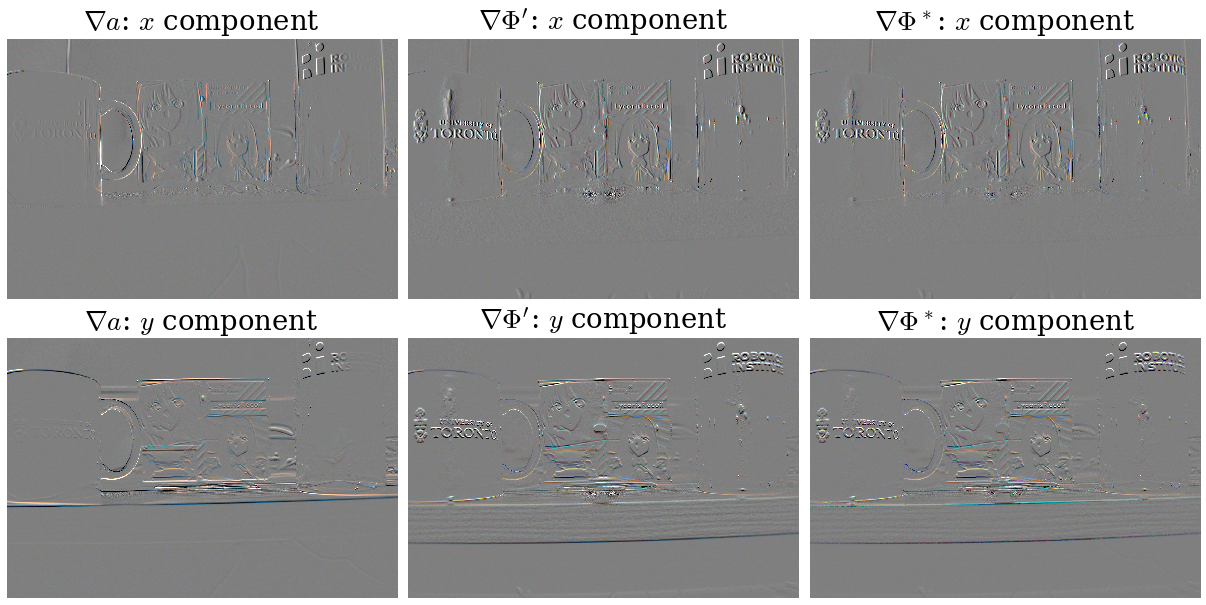
\includegraphics[width=\linewidth]{p3_glare_gradients.png}
\caption{Gradient fields of the ambient image, the flash image and the fused field ($\sigma=40$, $\tau_s=0.7$), shown per RGB channel as $0.5+g/0.3$ (mid-gray: zero gradient).}
\label{fig:p3p2grad}
\end{figure}
\begin{figure}[H]
\centering
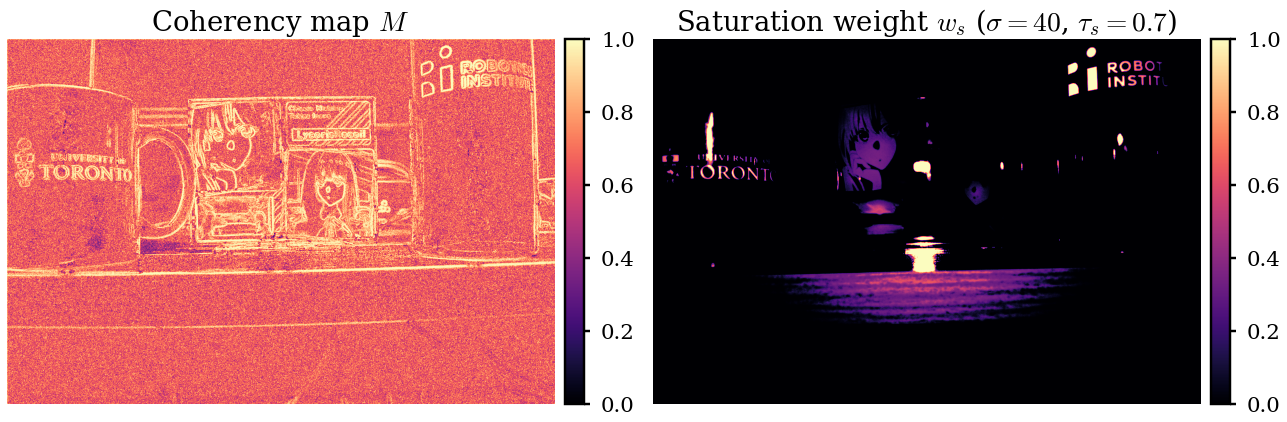
\includegraphics[width=\linewidth]{p3_glare_weights.png}
\caption{Coherency map $M$ and saturation weight $w_s$ with $\tau_s=0.7$. Besides the glare on the acrylic and the mug, $w_s$ also covers other bright flash regions: the white lettering on the mug and the bottle, and the front of the table.}
\label{fig:p3p2weights}
\end{figure}
\begin{figure}[H]
\centering
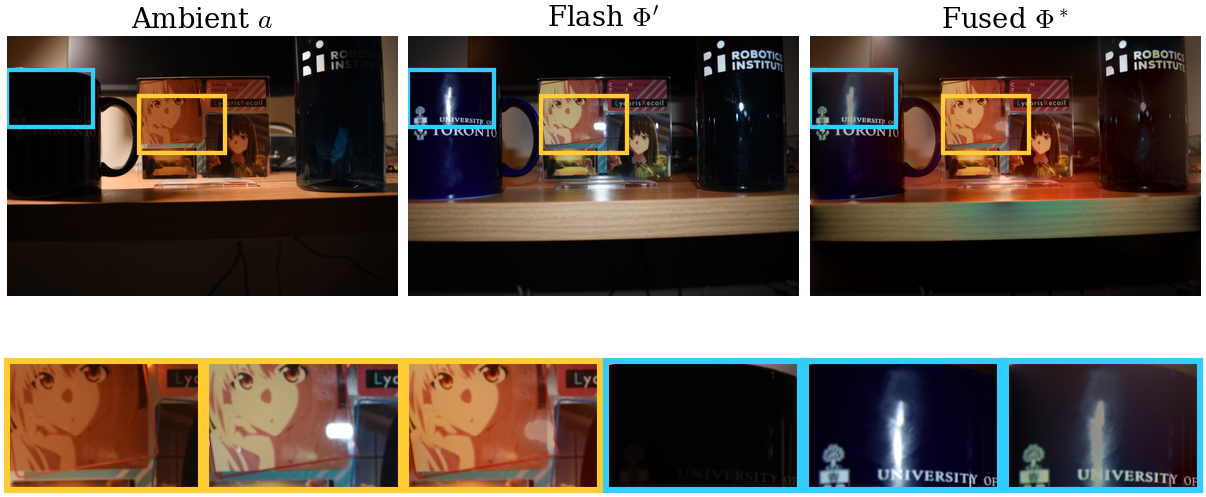
\includegraphics[width=\linewidth]{p3_glare_final.png}
\caption{Ambient image, flash image and fused result $\Phi^*$ with $\tau_s=0.7$, with zoomed views of the acrylic glare (yellow) and the mug (blue). The fused image keeps the lamp-lit cards from the ambient image and the mug and bottle from the flash image. The orange tint on the table front comes from the dark, noisy ambient gradients used where $w_s$ is large.}
\label{fig:p3p2final}
\end{figure}
\begin{figure}[H]
\centering
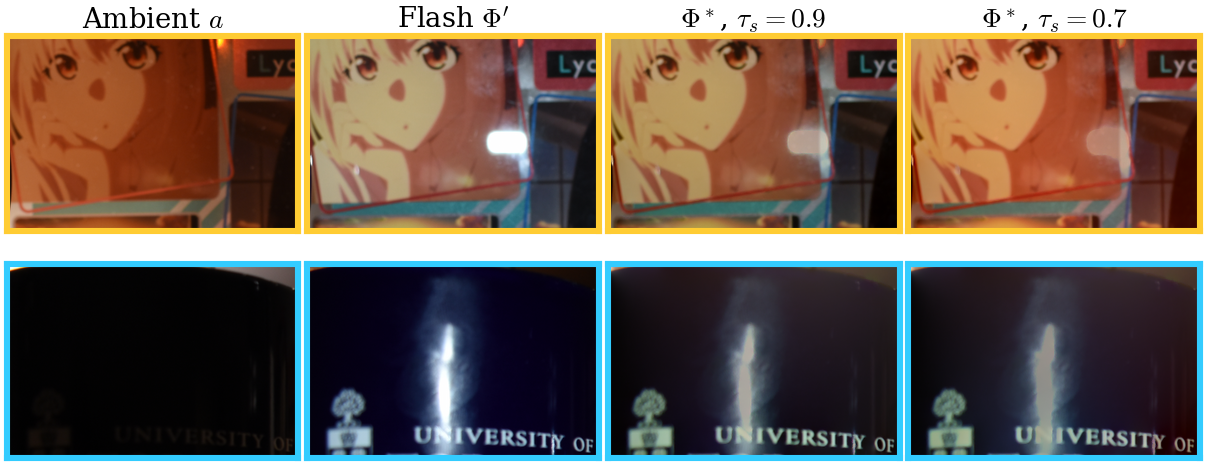
\includegraphics[width=\linewidth]{p3_glare_tau_compare.png}
\caption{Effect of $\tau_s$ on the two zoom regions. With the paper's $\tau_s=0.9$, a pale blob remains on the acrylic because only the saturated core is covered by $w_s$; with $\tau_s=0.7$ the halo is also replaced. The streak on the mug remains in both, because the mug is black in the ambient image.}
\label{fig:p3p2tau}
\end{figure}

%======================================================================
\clearpage
\section{Bonus: Reflection removal in flash/no-flash photography}
%======================================================================
\subsection*{Capture}
Following the Observation Deck scenario of Agrawal et al.\ (Section~4.1), I photographed a figure standing in front of a window at night, from inside the room. Both photographs were taken with the Nikon D3500 on a tripod at ISO 200 and $f/4$, with the room lights off. The ambient image was exposed for 15\,s: it shows the street, houses and parked cars outside, while the figure in front of the glass is dark. The flash image was exposed for 1/4\,s: the flash lights the figure and a white cup next to it, but these also reflect in the window glass, and the flash does not reach the scene outside.

\subsection*{Implementation}
I followed Equations~(13) and~(14) of the paper. The flash and ambient images are first added, $H=a+\Phi'$, so that both the figure and the outside are visible, but $H$ still contains the reflections. An underexposure map is computed from the ambient luminance $I$,
\begin{equation*}
w_{ue}=1-\tanh\big(\sigma(I-\tau_{ue})\big),
\end{equation*}
normalized to $[0,1]$, with $\sigma=40$ and $\tau_{ue}=0.1$. Where the ambient image is well exposed, the gradients of $H$ are projected onto the ambient gradients, which removes the component of the reflection gradients orthogonal to the ambient gradients (Equation~(9)); where it is underexposed, the gradients of $H$ are kept:
\begin{equation*}
\nabla\Phi^*=w_{ue}\nabla H+(1-w_{ue})\,(\nabla H\rightarrow\nabla a),\qquad
(\nabla H\rightarrow\nabla a)=\nabla a\,\frac{\nabla H\cdot\nabla a}{\|\nabla a\|^2}.
\end{equation*}
Each RGB channel is integrated with the CGD solver of Part~2. The removed component $(1-w_{ue})\big(\nabla H-(\nabla H\rightarrow\nabla a)\big)$ is integrated in the same way to visualize the reflection layer.

\subsection*{Discussion}
\begin{itemize}\setlength{\itemsep}{2pt}
\item \textbf{Scene design.} I placed a figure and a paper roll on the window sill, in front of the glass, and focused the camera on the house outside. In the flash image, both objects are lit by the flash and reflect in the glass, while the outside is not reached by the flash. I positioned the objects so that their reflections fall on the brightly lit street and house, because the method needs ambient gradients under the reflection: in an earlier attempt, the reflections fell on a dark tree and could not be removed at all.

\item \textbf{Result.} The method works partially: it makes the reflections fainter but does not remove them completely (Figure~\ref{fig:bonuscrops}). In the gradient visualization (Figure~\ref{fig:bonusgrad}), the edges of the reflected figure and paper roll are still visible in $\nabla\Phi^*$, only weaker than in $\nabla H$. This is expected from the projection: it only removes the component of a reflection gradient that is orthogonal to the ambient gradient, and since the reflection is unrelated to the scene outside, about half of its gradient energy is parallel and kept (53\% measured).

\item \textbf{Uniform reflections.} The reflected objects are fairly uniform, with few internal edges. Their reflection therefore acts mostly as a smooth brightening whose gradients are concentrated on its outline, and the method can only weaken that outline rather than remove the brightening itself. Using $H$ as the boundary values also leaves the outside slightly brighter than in the ambient image.
\end{itemize}

\begin{table}[!htbp]
\centering
\small
\begin{tabular}{ll}
\toprule
Step & Selected parameters \\
\midrule
Preprocessing & downsample to $1500\times1000$; no alignment (tripod) \\
Underexposure map & $\sigma=40$, $\tau_{ue}=0.1$ (values of Agrawal et al.) \\
Integration & $\epsilon=10^{-3}$, $N=5000$; initialization and boundary from $H$ \\
\bottomrule
\end{tabular}
\caption{Parameters for reflection removal.}
\label{tab:bonusparams}
\end{table}

\clearpage
\subsection*{Results}
\begin{figure}[H]
\centering
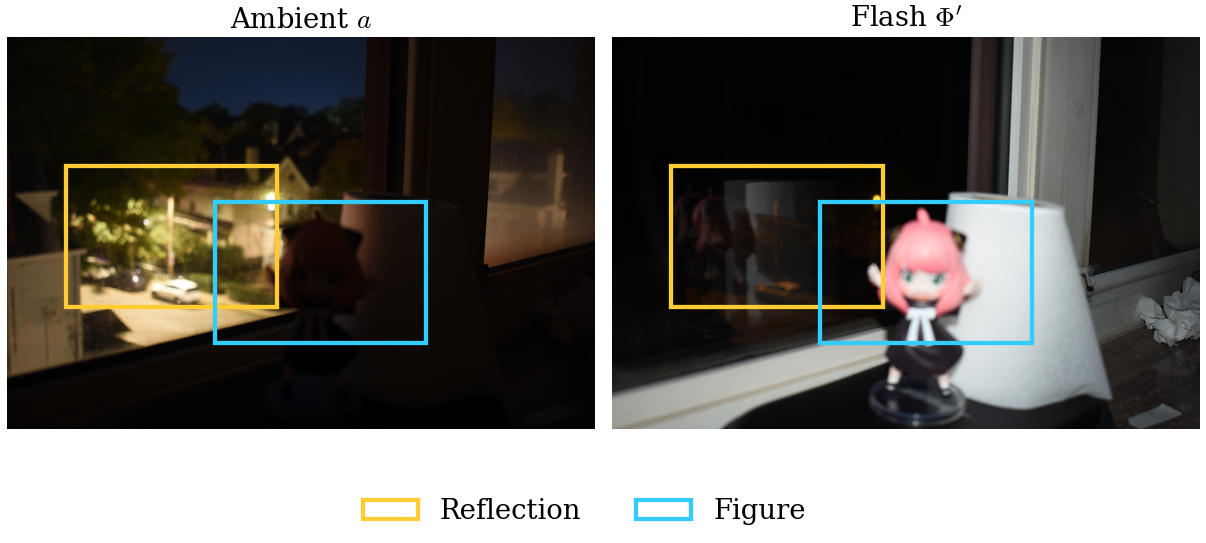
\includegraphics[width=\linewidth]{bonus_inputs.png}
\caption{Input pair: ambient image (ISO 200, 15\,s) and flash image (ISO 200, 1/4\,s), both at $f/4$. The boxes mark the zoom regions: the reflections of the figure and the cup over the lit street (yellow) and the figure (blue).}
\label{fig:bonusinputs}
\end{figure}
\begin{figure}[H]
\centering
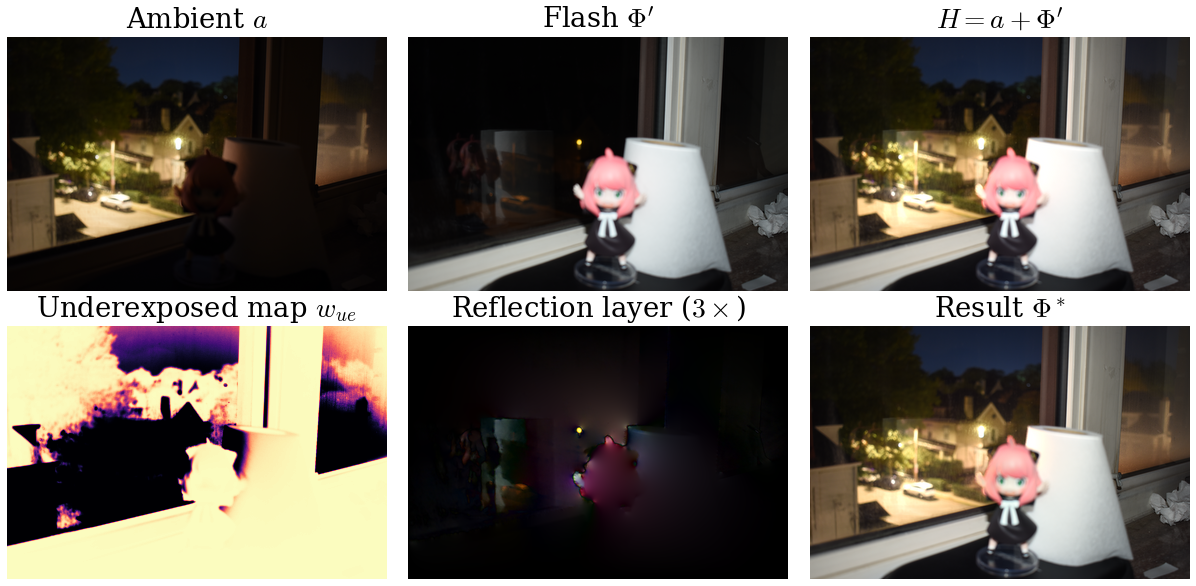
\includegraphics[width=\linewidth]{bonus_overview.png}
\caption{Top: ambient image, flash image and their sum $H$. Bottom: underexposure map $w_{ue}$ (close to 0 over the lit street and houses, where the projection is applied), the removed reflection layer (absolute value, $3\times$), and the result $\Phi^*$.}
\label{fig:bonusoverview}
\end{figure}
\begin{figure}[H]
\centering
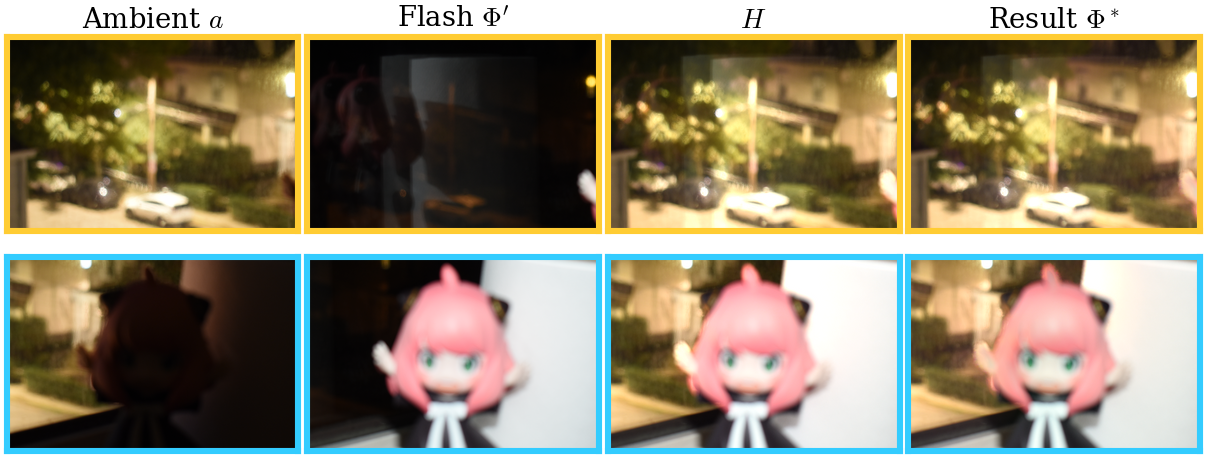
\includegraphics[width=\linewidth]{bonus_crops.png}
\caption{Zoomed views of the ambient image, the flash image, $H$ and the result $\Phi^*$. Top: the reflections of the figure and the cup over the lit street are reduced in $\Phi^*$. Bottom: the figure keeps the detail of the flash image.}
\label{fig:bonuscrops}
\end{figure}
\begin{figure}[H]
\centering
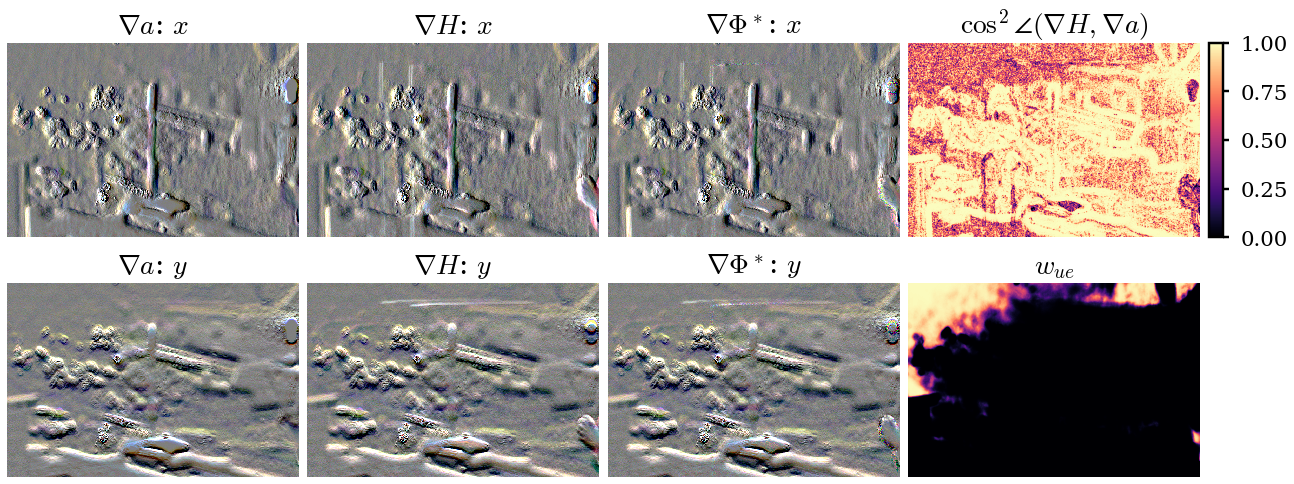
\includegraphics[width=\linewidth]{bonus_gradients.png}
\caption{Gradients in the reflection region (yellow box): $x$ and $y$ components of $\nabla a$, $\nabla H$ and $\nabla\Phi^*$, shown per RGB channel as $0.5+g/0.1$ (mid-gray: zero gradient); $\cos^2$ of the angle between $\nabla H$ and $\nabla a$ (the fraction of each gradient kept by the projection); and $w_{ue}$. The vertical edges of the cup's reflection are visible in $\nabla H$ and weaker in $\nabla\Phi^*$. Because the reflection is unrelated to the ambient scene, the projection keeps on average about half of its gradient energy (53\% measured).}
\label{fig:bonusgrad}
\end{figure}

%======================================================================
\clearpage
\section{Bonus: Gradient-domain non-photorealistic rendering}
%======================================================================
\subsection*{Task}
I implemented non-photorealistic rendering (NPR) in the gradient domain, following the idea of GradientShop: long, salient edges are emphasized and the remaining gradients (texture and shading) are suppressed, which produces a flat, cartoon-like rendering. The three examples are photographs of figures taken with my phone.

\subsection*{Implementation}
\begin{enumerate}\setlength{\itemsep}{0pt}
\item \textbf{Long-edge detection.} Instead of the long-edge detector of GradientShop, I use my own detector based on OpenCV's Canny edge detector. The image is first smoothed with my bilateral filter from Part~1 ($\sigma_s=3$, $\sigma_r=0.1$) so that texture does not produce edges. Canny is applied to the grayscale image with thresholds $0.66m$ and $1.33m$, where $m$ is the median intensity. Connected edge chains (8-connectivity, \texttt{cv2.connectedComponentsWithStats}) are kept only if their pixel count or bounding-box extent is at least 80 pixels. The resulting long-edge map is dilated with a $3\times3$ kernel and blurred with a Gaussian ($\sigma=1.5$) to obtain an edge weight $e\in[0,1]$.
\item \textbf{Gradient editing.} The target gradient field is $\mathbf{g}=\big(\alpha\,e+\beta\,(1-e)\big)\nabla u$, with $\alpha=2$ on long edges and $\beta=0.3$ elsewhere.
\item \textbf{Integration.} Each RGB channel is integrated with the CGD solver of Part~2 ($\epsilon=10^{-3}$, $N=3000$), with Dirichlet boundary values and initialization from the input image.
\end{enumerate}
The images are resized to a width of 1000 pixels (portrait photographs are rotated according to their EXIF orientation).

\textbf{Differences from GradientShop.} I replaced the long-edge detector with Canny plus a chain-length filter, and I use a pure Poisson formulation with fixed boundary values instead of GradientShop's combination of data and gradient constraints.

\subsection*{Discussion}

\begin{itemize}\setlength{\itemsep}{0pt}
\item \textbf{Effect.} The method strengthens the gradients on long edges and flattens the gradients elsewhere, which produces a cartoon-like rendering (Figures~\ref{fig:npr1}--\ref{fig:npr3}): the outlines detected by the long-edge detector become sharper, while the wood grain, the blurred background and the shading on the figures become flat.

\item \textbf{Parameters.} The effect is controlled by the two gains (Figure~\ref{fig:nprsweep}). A larger $\alpha$ makes the outlines more pronounced but also brightens large regions, and a smaller $\beta$ flattens the remaining regions more but also removes small details whose edges are too short to be kept, such as facial features.

\item \textbf{Artifacts.} Because each RGB channel is integrated separately with strongly scaled gradients, the channels drift by different amounts, which causes color shifts such as the green tint on the face in Figure~\ref{fig:npr3}. Applying $\alpha$ over a dilated and blurred edge band also produces a slight glow next to strong edges. Editing only the luminance and using a narrower edge band would reduce these artifacts.
\end{itemize}

\begin{table}[H]
\centering
\small
\begin{tabular}{ll}
\toprule
Step & Parameters \\
\midrule
Pre-smoothing & bilateral filter, $\sigma_s=3$, $\sigma_r=0.1$ \\
Canny & thresholds $0.66m$, $1.33m$ ($m$: median intensity) \\
Long edges & chain size or extent $\geq80$ px; dilation $3\times3$; Gaussian blur $\sigma=1.5$ \\
Gradient gains & $\alpha=2$ (long edges), $\beta=0.3$ (elsewhere) \\
Integration & $\epsilon=10^{-3}$, $N=3000$; boundary and initialization from input; width 1000 px \\
\bottomrule
\end{tabular}
\caption{Parameters for gradient-domain NPR.}
\label{tab:nprparams}
\end{table}

\clearpage
\subsection*{Results}
\begin{figure}[H]
\centering
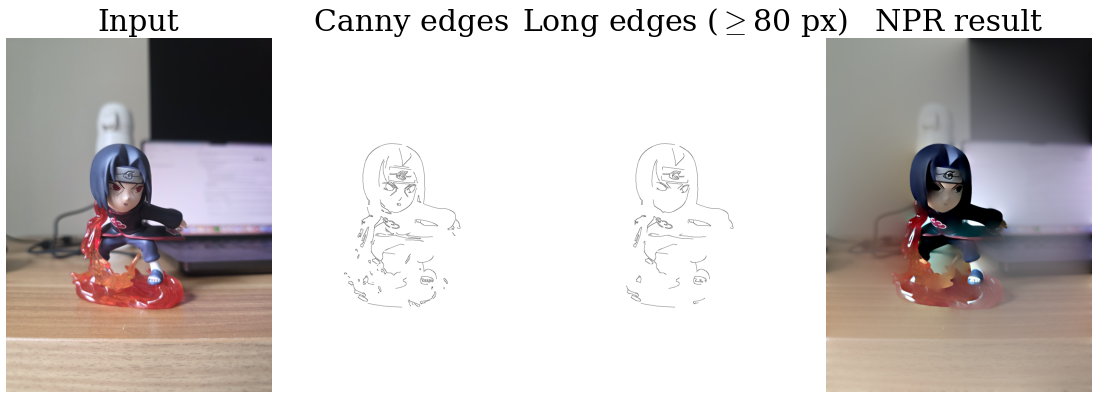
\includegraphics[width=\linewidth]{npr_photo1.png}
\caption{Example 1: input, Canny edges, long edges ($\geq80$ px) and NPR result.}
\label{fig:npr1}
\end{figure}
\begin{figure}[H]
\centering
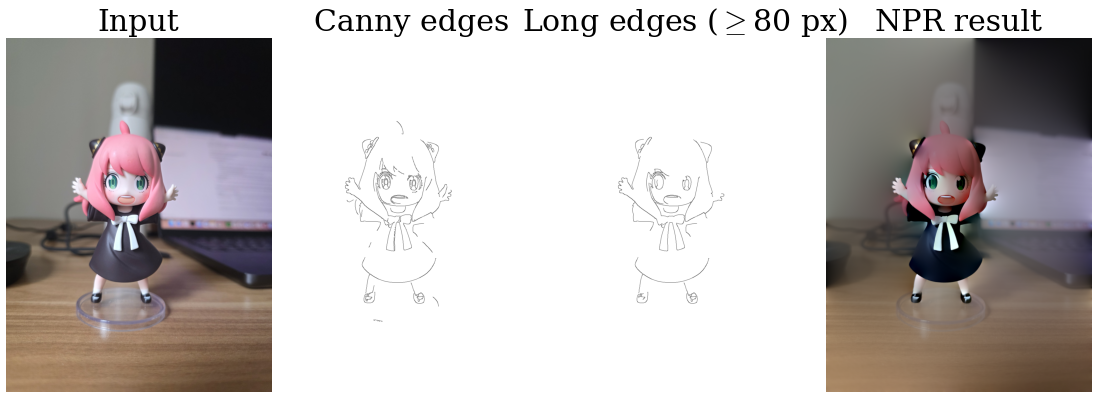
\includegraphics[width=\linewidth]{npr_photo2.png}
\caption{Example 2: input, Canny edges, long edges and NPR result.}
\label{fig:npr2}
\end{figure}
\begin{figure}[H]
\centering
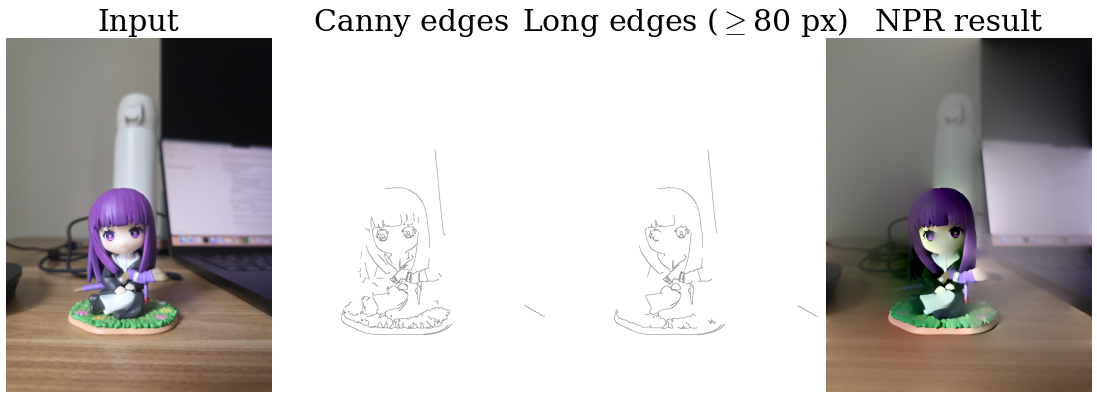
\includegraphics[width=\linewidth]{npr_photo3.png}
\caption{Example 3: input, Canny edges, long edges and NPR result.}
\label{fig:npr3}
\end{figure}
\begin{figure}[H]
\centering
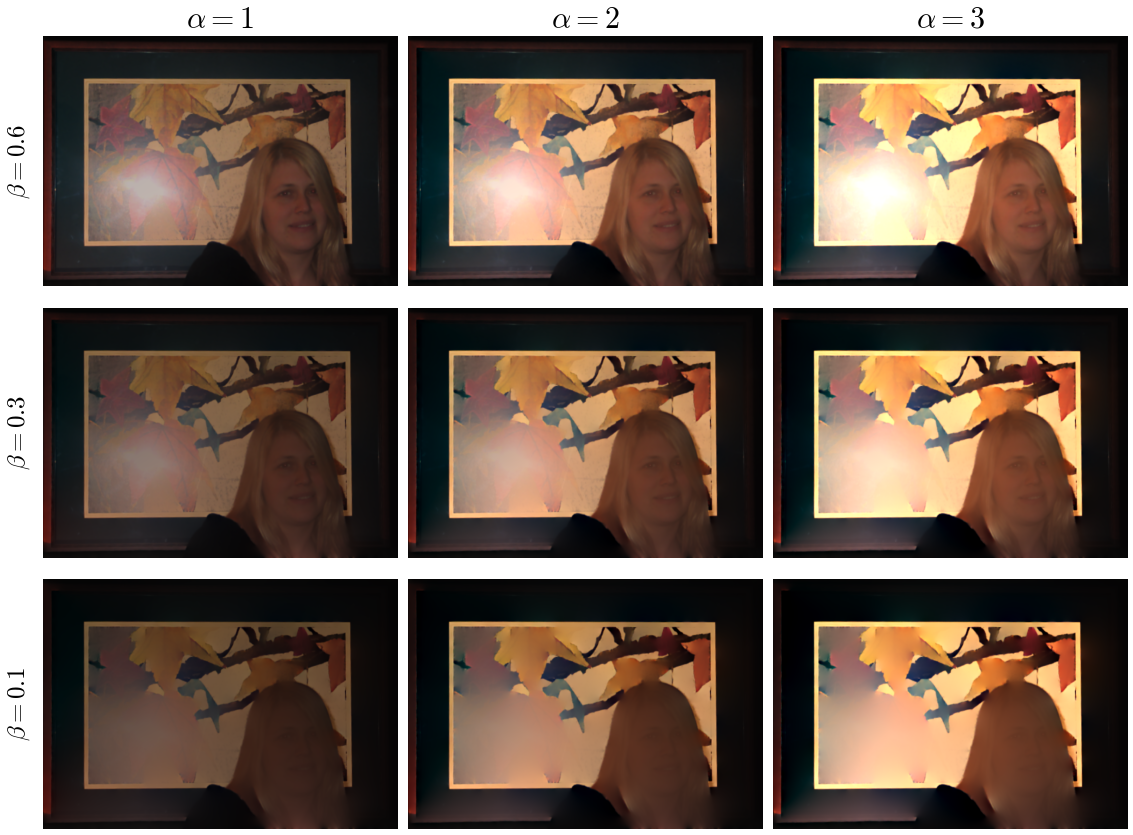
\includegraphics[width=0.85\linewidth]{npr_sweep_museum.png}
\caption{Effect of the gradient gains on the museum flash image (600 px wide; the minimum edge length is scaled accordingly): $\alpha\in\{1,2,3\}$ on long edges (columns) and $\beta\in\{0.6,0.3,0.1\}$ elsewhere (rows).}
\label{fig:nprsweep}
\end{figure}


%======================================================================
\clearpage
\section*{Acknowledgement}
The visualizations and the writing of this report were prepared in collaboration with Claude Code (Claude Opus 5.5).

\end{document}
